\documentclass{include/thesisclass}
% Main File - Based on thesisclass.cls
% Comments are mostly in English
% ------------------------------------------------------------------------------
% Further files in folder:
%  - include/cmds.tex (for macros and additional commands)
%  - include/kitlogo.pdf (for titlepage)
%  - lit.bib (bibtex bibliography database)
%  - include/titlepage.tex (for layout of titelpage)
% ------------------------------------------------------------------------------
% Useful Supplied Packages:
% amsmath, amssymb, mathtools, bbm, upgreek, nicefrac,
% siunitx, varioref, booktabs, graphicx, tikz, multicol





%% -------------------------
%% |    Thesis Settings    |
%% -------------------------
% english or ngerman (new german für neue deutsche Rechtschreibung statt german)
%\SelectLanguage{english}
% details on this thesis
\newcommand{\thesisauthor}{Isabel Haide}
\newcommand{\thesistopic}{Full event classification with data from the CMS/CASTOR calorimeter}
%\newcommand{\thesisentopic}{}
\newcommand{\thesislongtopic}{Very long and very detailed description of the very interesting thesis topic (only necessary for pdfsubject tag).}
\newcommand{\thesisinstitute}{Institut für Experimentelle Teilchenphysik}
\newcommand{\thesisreviewerone}{Prof. Dr. F. Bernlochner}
\newcommand{\thesisreviewertwo}{Dr. R. Ulrich}
\newcommand{\thesisadvisorone}{} % to use: enter names and uncomment in titlepg
\newcommand{\thesisadvisortwo}{}
\newcommand{\thesistimestart}{15.03.2018} % on titlepage
\newcommand{\thesistimeend}{01.07.2018} % on titlepage
\newcommand{\thesistimehandin}{01.07.2018} % on second page 'preamble'
\newcommand{\thesispagehead}{Bachelor Thesis: \thesistopic} % page heading





%% ---------------------
%% |    PDF - Setup    |
%% ---------------------
% This information will appear embed into the PDF file as meta data, but will 
% not be printed anywhere
\hypersetup
{
    pdfauthor={\thesisauthor},
    pdftitle={Bachelorarbeit: \thesistopic},
    pdfsubject={\thesislongtopic},
    pdfkeywords={kit,physik,bachelor,thesis,\thesisauthor}
}





%% --------------------------------------
%% |    Settings for Word Separation    |
%% --------------------------------------
% Help for separation:
% In German package the following hints are additionally available:
% "- = Additional separation
% "| = Suppress ligation and possible separation (e.g. Schaf"|fell)
% "~ = Hyphenation without separation (e.g. bergauf und "~ab)
% "= = Hyphenation with separation before and after
% "" = Separation without a hyphenation (e.g. und/""oder)

% Describe separation hints here:
\hyphenation
{
    über-nom-me-nen an-ge-ge-be-nen
    %Pro-to-koll-in-stan-zen
    %Ma-na-ge-ment  Netz-werk-ele-men-ten
    %Netz-werk Netz-werk-re-ser-vie-rung
    %Netz-werk-adap-ter Fein-ju-stier-ung
    %Da-ten-strom-spe-zi-fi-ka-tion Pa-ket-rumpf
    %Kon-troll-in-stanz
}




%% -----------------------
%% |    Main Document    |
%% -----------------------
\usepackage{lipsum} % for Lorem Ipsum text example
\begin{document}
    % Titlepage and ToC
    \FrontMatter
	\sffamily
    % coordinates for background border
\newcommand{\diameter}{20}
\newcommand{\xone}{-15}
\newcommand{\xtwo}{160}
\newcommand{\yone}{15}
\newcommand{\ytwo}{-253}




\begin{titlepage}
    % background border
    \begin{tikzpicture}[overlay]
    \draw[color=gray]
            (\xone mm, \yone mm)
      -- (\xtwo mm, \yone mm)
    arc (90:0:\diameter pt)
      -- (\xtwo mm + \diameter pt , \ytwo mm)
        -- (\xone mm + \diameter pt , \ytwo mm)
    arc (270:180:\diameter pt)
        -- (\xone mm, \yone mm);
    \end{tikzpicture}



    % KIT image and sign for faculty of physics
    \begin{textblock}{10}[0,0](4.5,2.5)
        
\includegraphics[width=.25\textwidth]{include/kitlogo.pdf}
    \end{textblock}
    \changefont{phv}{m}{n}    % helvetica
    \begin{textblock}{10}[0,0](5.5,2.2)
        \begin{flushright}
            \Large FAKULTÄT FÜR PHYSIK\\\thesisinstitute
        \end{flushright}
    \end{textblock}



    % horizontal line
    \begin{textblock}{10}[0,0](4.2,3.1)
        \begin{tikzpicture}[overlay]
        \draw[color=gray]
                (\xone mm + 5 mm, -12 mm)
          -- (\xtwo mm + \diameter pt - 5 mm, -12 mm);
        \end{tikzpicture}
    \end{textblock}



    % begin of text part
    \changefont{phv}{m}{n}    % helvetica
    \centering



    % thesis topic (en and ge)
    \vspace*{3cm}
    \Huge\thesistopic\\
%    \huge(\thesisentopic)\\



    % author name and institute
    \vspace*{2cm}
    \Large Bachelorarbeit\\von\\
    \vspace*{1cm}
    \huge\thesisauthor\\
    \vspace*{1cm}
    \Large am \thesisinstitute



    % possible frontimage - thanks to JabberWok
    % for publishing the img under GNU Document License
    \vspace*{1.5cm}
    %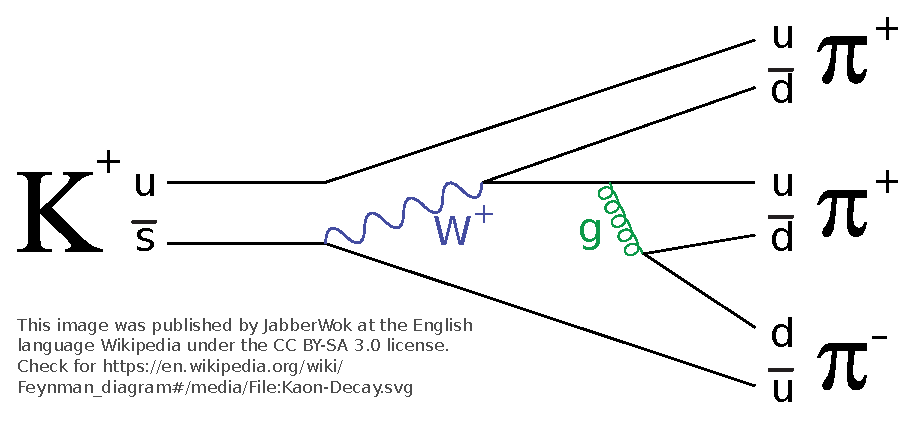
\includegraphics[scale=0.7]{./include/frontimage.eps}\\



    % examiners (Referenten)
    \vspace*{1.5cm}
    \Large
    \begin{center}
        \begin{tabular}[ht]{l c l}
        \iflanguage{english}{Reviewer}{Referent}: 
            & \hfill & \thesisreviewerone\\
        \iflanguage{english}{Second Reviewer}{Korreferent}: 
            & \hfill & \thesisreviewertwo\\
        % uncomment if you want to provide info on your advisors
        %\iflanguage{english}{Advisor}{Betreuender Mitarbeiter}: 
        %    & \hfill & \thesisadvisorone\\
        %\iflanguage{english}{Second Advisor}{Zweiter betreuender Mitarbeiter}: 
        %    & \hfill & \thesisadvisortwo\\
        \end{tabular}
    \end{center}



    % working time
    \vspace{1cm}
    \begin{center}
        \large{{Bearbeitungszeit}: \thesistimestart \hspace*{0.25cm} -- %
                                   \hspace*{0.25cm} \thesistimeend}
    \end{center}



    % lowest text blocks concerning the KIT
    \begin{textblock}{10}[0,0](4,16.8)
        \tiny{KIT -- Universität des Landes Baden-Württemberg und nationales %
              Forschungszentrum in der Helmholtz-Gemeinschaft}
    \end{textblock}
    \begin{textblock}{10}[0,0](14,16.75)
        \large{\textbf{www.kit.edu}}
    \end{textblock}
\end{titlepage}

    \chapter*{Erklärung zur Selbstständigkeit}
Ich versichere, dass ich diese Arbeit selbstständig verfasst habe und keine %
anderen als die angegebenen Quellen und Hilfsmittel benutzt habe, die %
wörtlich oder inhaltlich übernommenen Stellen als solche kenntlich gemacht und %
die Satzung des KIT zur Sicherung guter wissenschaftlicher Praxis in der %
gültigen Fassung vom 17.05.2010 beachtet habe.\\

\vspace{1cm}

\renewcommand{\arraystretch}{0} % for spacing in the tabular environment

\begin{flushright}
	\begin{tabular}{rr}
		Karlsruhe, den \thesistimehandin, & \hspace*{5cm}\\[0mm]
		\cline{2-2}\\[2mm]    % the last line has height 2mm due
		& \thesisauthor       % to \arraystretch=0
	\end{tabular}
\end{flushright}

\vfill

\begin{flushright}
	Als Ansichtsexemplar genehmigt von\\
	\vspace{1cm}
	\begin{tabular}{rr}
		Karlsruhe, den \thesistimehandin, & \hspace*{5cm}\\[0mm]
		\cline{2-2}\\[2mm]    % the last line has height 2mm due
		& \thesisreviewerone  % to \arraystretch=0
	\end{tabular}
\end{flushright}

\renewcommand{\arraystretch}{1}

\cleardoublepage

	\section*{Abstract}

In current particle physics research the search for new particles is a major part in most experiments. To be able to correctly separate unknown from known events a full event classification is necessary. In this thesis a full event classification with the CASTOR calorimeter as part of the CMS detector at CERN is done. The classification is made with the help of convolutional neural networks, treating the input data as images. Simulated events generated by the Monte Carlo generators PYTHIA8 and EPOS are used. To simplify the analysis the events are split into only two categories, electromagnetic events containing electrons and photons with their respective antiparticles and hadronic events. Furthermore only single particles with no other particle crossing CASTOR during this event or isolated particles with a distance of at least $\Delta$R = 0.8 to the next particle are included in the training data. The trained network is evaluated on real data measured by CASTOR. As real data contains only a small amount of single or isolated events the classification could not correctly separate the categories. If the predicted possibility of one event belonging to one category was 80 \% or higher, sampled events are correctly identified. With a better performance, reachable by more refined networks or preprocessed data, such an event classification could possibly reach human performance.  

\vspace{2cm}

In der aktuellen Teilchenphysikforschung ist die Suche nach neuen Teilchen eines der größten Aufgabenfelder. Um eine korrekte Trennung zwischen bekannten und unbekannten Events zu ermöglichen, muss eine vollständige Eventklassifizierung möglich sein. In dieser Arbeit ist eine solche Klassifizierung am CASTOR-Kalorimeter als Teil des CMS Detektors am CERN durchgeführt worden. Dafür wurde ein neuronales Netz mit Convolutional Layers verwendet, welches die Daten als Bilder interpretierte. Für das Training des Netzwerkes wurden von den Monte Carlo Generatoren PYTHIA8 und EPOS generierte Events verwendet. Um die Analyse zu vereinfachen, sind die Events in zwei Kategorien aufgeteilt, elektromagnetische Events mit Elektronen und Photonen und deren Antiteilchen und hadronische Events. Zudem werden nur isolierte Teilchen in die Trainingsdaten aufgenommen, welche entweder einen Mindestabstand von $\Delta$R = 0.8 zu ihrem nächsten Nachbarn hatten oder ohne weiteres Teilchen innerhalb von CASTOR detektiert wurden. Das trainierte Netzwerk wird dananch an echten Daten getestet. Da diese nur zu einem geringen Anteil isolierte Events enthalten, kann das Netzwerk diese Daten nicht vollständig den einzelnen Kategorien zuordnen. Nur wenn die vorhergesagte Wahrscheinlichkeit bei über 80 \% liegt, sind ausgewählte Events richtig klassifiziert. Mithilfe von besser zugeschnittenen neuronalen Netzen oder vorverarbeiteten Daten kann das Netzwerk verbessert werden, um möglicherweise eine Eventklassifizierung zu vereinfachen.
\cleardoublepage
	
    \begingroup \let\clearpage\relax    % in order to avoid listoffigures and
    \tableofcontents                    % listoftables on new pages
    \listoffigures
    \listoftables
    \endgroup
    \cleardoublepage



    % Contents
    \MainMatter

    \chapter{Introduction}
    One objective of the Large Hadron Collider (LHC) at CERN was to be able to produce and identify new particles at very high energies. Several different detectors have been installed that could possibly observe such particles \cite{atlas} \cite{cmscollab}.
The CASTOR calorimeter is a very forward detector, located at the edge of the CMS detector at the LHC. CASTOR can provide information on a number of topics. One of these is the hypothesis of strangelets, a theoretical particle consisting of up, down and strange quarks \cite{strangelet}. Particles with a small number of strange quarks are unstable as the strange quark decays into the lighter quarks via the weak interaction. The \enquote{strange matter hypothesis} states that composite particles with a higher number of strange quarks and roughly the same number of up and down quarks may become stable. As such particles have a very high mass, they could mostly be detected in the very forward region of the CMS detector. Thus, CASTOR was constructed to search for strangelets \cite{strangeletcastor}. To find such events it is crucial to correctly identify characteristic signatures made by known backgrounds and to separate them from possible unknown signals. \newline
Neural networks have many applications nowadays. They are used mostly when very large amounts of data are available and a distinctive pattern can be picked out. Particle physics is therefore a prime field for the application of neural networks \cite{dnnparticle1}\cite{dnnparticle2}\cite{dnnparticle3}. With the help of Monte Carlo simulations features can be learned and detected. In this thesis a neural network is developed to correctly identify and differentiate particle signatures in CASTOR. If this network can correctly classify known events, possible new particle signatures can be found as excess over the background after the classification. A further possibility could be to include the theoretical signature of for example a strangelet and to specifically look for such events in real data. \newline
The event classes given to the network in this thesis consisted of electromagnetic particles, electrons and photons, hadronic particles, such as pions and protons, and background. To further simplify the work of the network, only isolated or single particles are selected as events. With this selection three different data sets have been composed, one containing isolated particles, one single particles and the last being a binary set with only the electromagnetic and hadronic class, omitting the background completely. To train the network Monte Carlo-generated proton proton collisions ad $\sqrt{\mathrm{s}} = 13 \,$TeV generated by PYTHIA8 and EPOS are used. The network is then tested on actual CASTOR events. In the end the application and functionality of the network is also evaluated on low-luminosity data recorded in June 2015. 
    \chapter{The detector}
    \section{The CMS Experiment}
The large hadron collider (LHC) at Geneva, Switzerland, is build to accelerate protons to very high velocities. In two adjacent beamlines, proton bunches travel in opposite directions around the ring. Eventually, those bunches collide in dedicated crossing points, which are surrounded by seven detectors. One of those detectors is the CMS experiment (see fig. \ref{cms}). CMS stands for Compact Muon Solenoid, a general-purpose detector built in several layers. In the centre of the detector is the interaction point where the proton-proton collisions occur.

Around this interaction point the different kinds of detectors are build in layers around the beamline. Those track and identify the particles produced by the proton-proton collision. The name giving solenoid magnet produces a magnetic field of 3.8\,T to curve the paths of the particles inside the detector. Inside the magnet volume is the tracker to identify the momentum of the particle and the electromagnetic followed by the hadronic calorimeter to measure the energy of various particles.  To detect muons, which penetrate the iron of the calorimeters, muon chambers are installed outside of the CMS magnet. \cite{CMS}

To be able to identify the angle of a particle relative to the beam axis, the pseudorapidity  ${\eta \equiv - \ln \left[ \tan \left( \frac{\theta}{2} \right) \right]}$ is used. Here $\theta$ gives the angle between the particle \mbox{impuls $\vec{p}$} and the positive direction of the beam axis.Typically particles with a high pseudorapidity are not measured, as they escape the detector alongside the beam. 
\begin{figure}
\centering
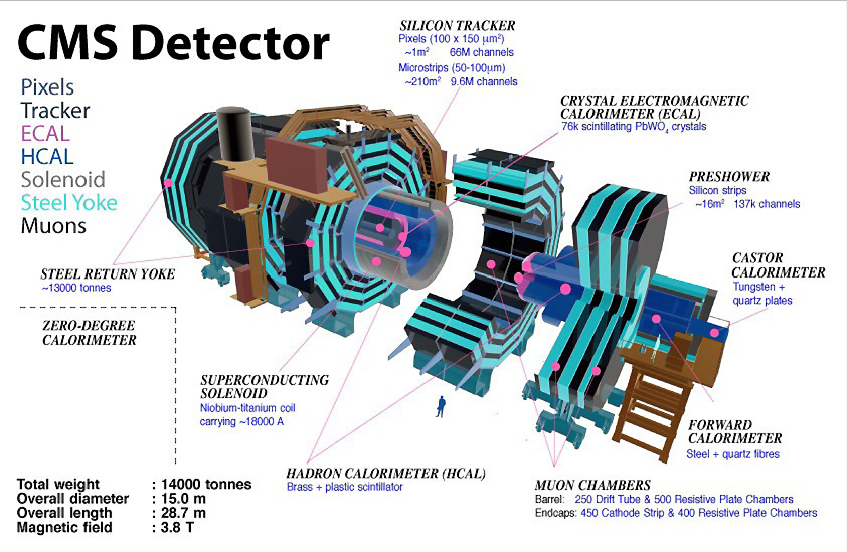
\includegraphics[scale=0.4]{cms_with_castor_drawing.jpg}
\caption{The CMS detector including its layers. The beam line is surrounded by the tracker and various calorimeters, as well as the superconducting solenoid and the muon chambers. CASTOR is located at the far right. (source: \cite{CMSbild}).}
\label{cms}
\end{figure}

\section{The CASTOR Calorimeter}

The CASTOR calorimeter is part of the CMS detector. CASTOR stands for \enquote{Centauro And Strange Objects Research}. It is a very forward detector, covering the pseudorapidity range of -6.6 < $\eta$ < -5.2 . CASTOR is a electromagnetic and hadronic calorimeter which utilizes the Cherenkov effect to detect and classify particles. The calorimeter is divided into 16 sectors in azimuth and has 14 segments of readout units, or modules, along the longitudinal axis. The total number of channels is therefore 224. The 14 modules belonging to one sector are also called a tower.
The first two modules of every tower are electromagnetic readout units (EM modules) with a thickness of 7 mm each, which combine to 20.12 X$_0$. The remaining 12 modules form the hadronic calorimeter (HAD modules) with a thickness of 14 mm each, therefore with a length of 9.504 $\lambda_{\mathrm{I}}$. 
Its active material are quartz plates (2 mm thickness in the EM modules, 4 mm in the HAD modules) with tungsten absorbers inbetween (5 mm in EM, 10 mm in HAD modules). The entire detector has a length of 10.30 $\lambda_{\mathrm{I}}$, an inner radius of 3.7 cm and an outer radius of 14 cm. Outside of that the readout and infrastructure components are located, restricted to an outer radius of 30 cm given by the radiation shielding of CMS. Since CASTOR is therefore between the beam line and the radiation shield, it had to be built to withstand high radiation levels as well as high magnetic fields from the CMS magnet. 



If a particle produced by the initial collision at the interaction point reaches the calorimeter, it initiates a shower of secondary particles. These produce Cherenkov light, which can be detected by CASTOR. The quartz plates and tungsten absorbers have a 45$\degree$ inclination in respect to the beam axis to maximize the production of Cherenkov light. The photons produced by the Cherenkov effect are then transmitted to photomultiplier tubes (PMTs) with the aid of aircore lightguides. The PMTs transform the light into an electric signal. Each PMT corresponds to one of the 224 modules.
As the detector does not compensate the effect that electromagnetic particles produce more Cherenkov photons and therefore a higher energy response than hadronic particles, it is called a non-compensating calorimeter.



During high luminosity runs with p-p collisions CASTOR has to be removed from the beam line. As the detector is positioned very near the interaction point and due to its geometry it is impossible to evaluate pileup events. For that reason, to reduce the amount of radiation and to avoid back scattering of particles into CMS CASTOR is only installed during runs with low luminosity, where the number of collision per bunch crossing is $\approx$ 1. For runs with low luminosity or Pb-Pb collisions it has to be easily reinstalled. For this reason the detector can be split into two halves, each containing eight towers, to be removed from the beam line and then lifted up by a crane. \cite{castor}

\begin{figure}
\centering
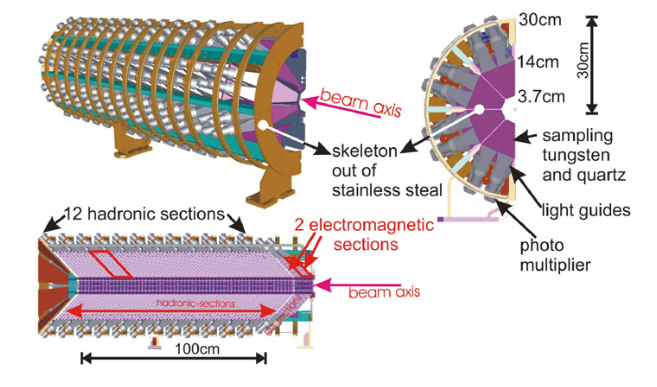
\includegraphics[scale=0.8]{castor.png}
\caption{The CASTOR	calorimeter. It is built in two parts around the beam line, with eight towers respectively, each tower containing two electromagnetic and twelve hadronic readout units. The readout units have a $45\degree$ inclination respective to the beam axis to maximize light production (lower left). (source: \cite{castorbild}).}
\end{figure}

    \chapter{Neural networks}
    Artificial neural networks (ANN) were inspired by the idea of developing programs that are able to learn how to perform certain tasks by getting examples. Neural networks generally don't have any task-specific rules implemented, they learn the important features by themselves. 

The basic idea was to model the neurons in a biological brain. Such artificial neurons (also called connected units or nodes) are linked to each other and transmit signals. The neuron receives the signal and combines it with a certain weight and bias before sending it to the next connected unit. The weight and the bias are free parameters which have to be optimized by the network itself. 
In ANNs, nodes are combined into layers. The input data is processed by several layers connected to each other. Each layer is typically trained to extract a certain feature of the input data to yield the required information at the end. 

Neural networks are mostly used for two different kinds of analysis. The first one is the prediction of a continuous variable, which is called a regression problem. The second, which is specified here, is the problem of identifying an input as part of a class, called a classification model.
In classification problems the training is typically supervised. The network is given input data and corresponding label vectors which state to which category the respective input belongs. False labelling is penalized and leads to weight and bias adjustments.

Training a network means giving examples of the task and evaluating the performance of the network. This evaluating is done through backpropagation. The input propagates through the network until it reaches the output layer. There it is compared to the actual output vector. The difference between these two or the classification error is given by a loss function. This error is then propagated backwards through the network until every neuron has an associated error value. Through this value the weight and bias of the corresponding neuron is then changed to improve the performance of the network. 

As updating the weights after every input sample is inefficient and makes the loss function very noisy, several samples are combined in one batch or minibatch. The training values are averaged over the sample and the network learns more general features. 

Typically the available input data is limited and can not be easily generated. The network therefore uses the same data several times during the training. One training session which uses the entire data set exactly once is called an epoch. To fully train a ANN several hundred epochs are needed. To prevent the network only being able to classify the training data correctly a small part of it is being split off. This data set is called the validation data. After every epoch the network evaluates its progress on the validation data which has not been used during training. This secures an independent evaluation.  

In contrast to the free parameters set by the network, hyperparameters have to be specified before training starts. Different kinds of networks have different hyperparameters, one for example being the size of the minibatch. Optimized hyperparameters contribute significantly to the success of the network. \cite{Bishop2016}


\section{Image recognition}
Image recognition has always played a huge part in the development of neural networks. Current state-of-the-art networks in image recognition have now reached human or even superhuman performance. Image recognition with neural networks is normally placed within the \enquote{deep learning} category. Such architectures include successive layers with nonlinear processing units. Each layer is connected to its predecessor and uses the output of the latter as input. This enables the network to learn different features, higher layers then correspond to higher levels of abstraction. 

 The problem with conventional multilayer perceptrons are the computing power needed. In conventional ANNs the neurons are fully connected, meaning that every node in one layer is connected to every node in the layer before and after. The number of weights per node is equivalent to the product of width, height and colours of the picture. They therefore scale very badly to higher resolution images. Fully connected layers also do not take localized characteristics into account. In image recognition neighbouring pixels are more important than those far apart.
Convolutional neural networks (CNNs) can solve both problems and are currently the best performing networks \cite{imagenet}.



\section{Convolutional neural networks}

\begin{figure}
\centering
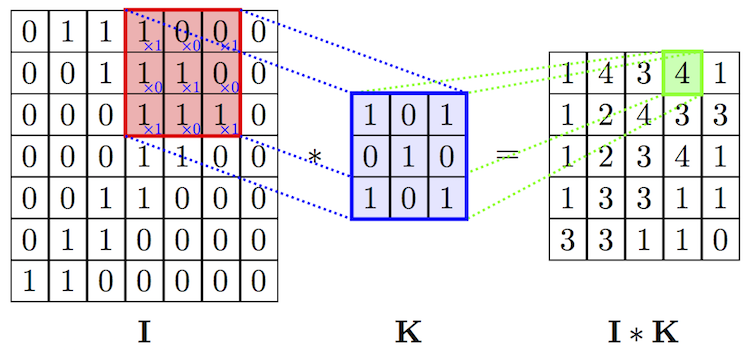
\includegraphics[scale=1.5]{convolve.png}
\caption{A convolutional layer with its kernel. The elements of the kernel are also called a filter. The kernel moves across the whole input data on the left. The right matrix is the product of input and kernel. \cite{convwindow}}
\label{convwindow}
\end{figure}
A convolutional neural network contains several layers in which one input sample is processed in small receptive fields (as seen in fig. \ref{convwindow}). These receptive fields are most often called kernel or filter. One neuron in the layer corresponds to only this part of the input image in width and height but gets the whole depth of the input volume. The dot product between the entries of the kernel and the input is computed and sent to the neuron. The filter values or weights are free parameters of the network that have to be optimized. For different sets of parameters different features can be detected.
The map of neurons is called the activation map. As several input pixels are passed on to one neuron, the size of the input data gets gradually smaller while it is being processed by the network.

Convolutional neural networks are dominated by three different features which make them ideal for image recognition. The first is the 3D volume of neurons, where they are classified in three dimensions, width, height and depth of colour. This ideally represents a picture. The second is the application of spatial locality. One neuron of a following layer is only connected to a small part of neurons in its predecessor. Therefore the network learns to recognize local patterns. With many such layers stacked the patterns learned get increasingly more global, the first one only recognizing lines, while the last one identifies complete features such as \enquote{cat}, \enquote{dog} or \enquote{mouse}.
At last a convolutional neural network takes translational invariance into account. To classify an image correctly, the position of the object in the image is not important. Therefore all neurons in one convolutional layer share the same weights and bias, that means, the same filter is applied while forwarding the signal. Thus one layer always recognizes the same feature, regardless of its position in the image \cite{lecunimage}. 

The hyperparameters for this kind of ANN, which have to be manually tuned, are firstly the size of the convolutional window. If a size of one in width and height is chosen, the window only takes one pixel into account. A bigger size means more information is being observed. The bigger the window the less localized the features detected are. Smaller windows mean more computing power needed, and may not be able to detect larger objects, especially in high resolution pictures. At times it may be advantageous to choose a non-symmetrical kernel size.

The second hyperparameter is the depth of the output volume. It is possible to choose how often a kernel with a new set of weights will be used on the input data or further on in the network. As one kernel with a set of weights is also called a filter, the number of filters can be manually tuned. The more filters are being used, the more free parameters the network has. This can be beneficial as more details can be learned by the network but also disadvantageous as overfitting, which is explained later, is more likely to occur.

If the kernel size is chosen, the stride must be finetuned as well. If the stride is one, then the window only moves one pixel in one direction each time. A high overlap of kernel windows occurs which also produces a large output volume. This can significantly increase the computing time. If the kernel size is large, than a higher overlap is helpful.

When the size of the input volume is not a multiple of the kernel size window, then the output dimensions differ from those of the input. Most of the time it is helpful to pad the input volume with zeros at the edges to preserve the spatial size of the input while going through layers. It is also beneficial to minimize edge effects. \cite{lecun-89e}

\section{Overfitting}
Overfitting is a potential problem of deep-learning networks. By choosing layers with a high number of learnable weights and biases, the number of free parameters is very high compared to the actual number of features learnable. Therefore a network is prone to overfit the training data, performing very well during the training but failing while validating on other data (fig. \ref{accuracy}). 

\begin{figure}
\centering
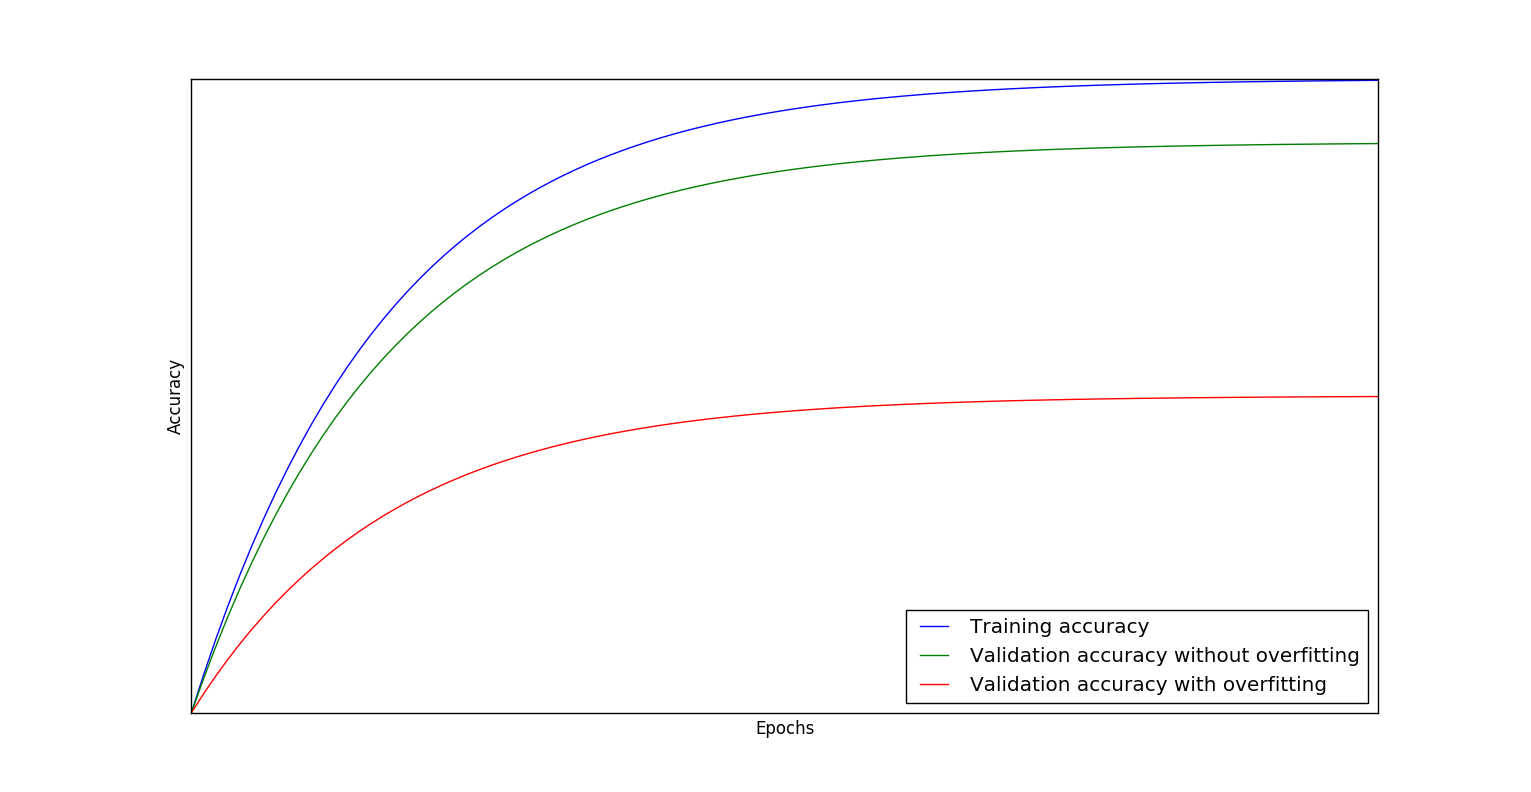
\includegraphics[scale=0.35]{overfittingacc.png}
\caption{Training and validation accuracy. The validation accuracy follows the training accuracy well if there is little or no overfitting. In the case of strong overfitting the validation accuracy increases very little or even decreases during the training.}
\label{accuracy}
\end{figure}
One method to address the problem of overfitting is \enquote{max pooling}. Max pooling also reduces the spatial size, thus limiting the amount of computational power needed. The general idea is that only the rough location in comparison to others of the feature detected is needed, so the input is downsampled with the help of a non-linear function. The working principle is the same as in a convolutional layer. A kernel window moves over the input without overlapping. In every region the activation numbers of the included pixels are compared. The maximum is determined and only this pixel is forwarded to the next layer. For example, in the case of a 2x2 kernel window, the spatial size is reduced by 75 \%, while the depth dimension stays the same. As the network cannot fit parameters to very detailed features, it has to pick up general features, which help correct classification. 

Another method to reduce overfitting is dropout. With dropout a input unit is set to zero before being forwarded to the next layer with a possibility $p$. This is the same as to set every weight of one neuron to zero. This is done with after every minibatch of samples, which is tantamount to every parameter update of the network. This forces the CNN to learn more robust features to better generalize the data analysis. Dropout also cuts down on computational time. 

\section{Activation functions}
Deep neural networks need two different kinds of activation functions. The first one is to propagate the signal through the network. After the product between the input signal and the weight of one neuron is computed, the outcome is put into the activation function. Only if a nonlinear activation function is used, non trivial problems can be solved with only few nodes. The activation function is applied after every layer, meaning that every output signal is put into relation with the help of the function. The current best working activation function is the ReLu function. ReLu stands for rectified linear unit. It is calculated by
\begin{equation}
f(x) = \mathrm{max} (0,x)
\end{equation}
with x as the input signal. Negative signals are therefore always set to zero while propagating through the network. Other activation functions are for example the sigmoid function or the tangens hyperbolicus. Unlike the ReLu function, those functions saturate when dealing with very high input signals and therefore perform worse.

The second activation function is needed at the output layer, the last layer in the network. Most deep neural networks are multi-class networks. Multi-class means that the output is not simply signal or background but identifies the input as belonging to one class of several. That means that the output activation function calculates the probability of belonging in each class in correlation to every other probability. A usual activation function in this case is the softmax function. The softmax function calculates a n-dimensional vector of random real values to a n-dimensional vector, where every number lies between 0 and 1 and the sum of all entries is 1. It is calculated by
\begin{equation}
\sigma (\vec{z})_{j} = \frac{\mathrm{e}^{z_j}}{\sum_{k=1}^{n} \mathrm{e}^{z_k} } \quad .
\end{equation}
The vector $\vec{z}$ is the output vector of the neural network, which corresponds after the application of the activation function to $\sigma (\vec{z})_{j}$, the probability of the input belonging to the corresponding classes.
The softmax function cannot be applied if the network is not only multi-class, but also multi-label. The categories in a multi-label network are not mutually exlusive. One input can therefore be classified into several different categories, their probability to fit is not correlated to each other. In this case the beforementioned sigmoid activation function can be used. This function also squashes a vector of real numbers to a vector of real numbers between 0 and 1. In this case the sum of all numbers does not have to be 1. The output $\sigma (\vec{z})_{j}$ is the independent probability of the input data belonging to class j without taking the other classes into account. The function looks like
\begin{equation}
\sigma (\vec{z})_{j} = \frac{1}{1 + \mathrm{e}^{z_j}}  
\end{equation}
with $\mathrm{e}^{z_j}$ as the output vector of the network.
Assigning a class to the input data is normally done by selecting those entries which have a number higher than 0.5, meaning a probability higher than 50\% of belonging to that class. 
\section{Loss functions}
Loss functions are a way to track the progress while training a neural network. A loss function assigns a real number to the difference between real and estimated class labels of the input, which should be minimized. During training the network changes the weights of the neurons according to the increase or decrease of the loss function. For a specific problem it is important to use a suitable loss function. For classification problems such as image recognition with more than two classes, either categorical or binary crossentropy can be used. In machine learning cross entropy is the same as logistic loss. It is calculated by
\begin{equation}
f(x) = y_{\mathrm{true}} \cdot \mathrm{ln} (y_{\mathrm{pred}}) + (1 - y_{\mathrm{true}}) \cdot \mathrm{ln} (1 - y_{\mathrm{pred}})
\end{equation}
where $y_{\mathrm{true}}$ is the true label vector of the input and $y_{\mathrm{pred}}$ the label vector of the prediction of the network.

The difference between categorical and binary crossentropy is only the way in which it is applied. With categorical crossentropy, the whole vector is compared. If only one entry differs, it is considered falsely labeled. This is useful in multi-class problems, where the labels are mutually exclusive. With multi-label problems, binary crossentropy works better. Binary crossentropy compares every label separately, therefore not penalizing one incorrect label so much. 

\section{Optimization algorithms}
To minimize the loss function the neural network has to update its weights and biases during training. This updating is done through an optimization algorithm. To find a minimum of the loss function it is possible to evaluate the gradient of the function. The updating of the network is then proportional to the negative of the gradient. This is an iterative algorithm which finds the steepest descent to a local minimum. The size of the steps taken in the direction of the descent is also called the learning rate. The learning rate is a hyperparameter which has to be optimized to get best training results. 

To compute the gradient for the whole training data takes very long. To shorten the time and computing power needed stochastic gradient descent (SDG) is implemented. SDG uses only one stochastically chosen example to compute the gradient and update the parameters. This can of course result in very varying parameter updates. To prevent this the gradient is computed not over one sample, but over a whole batch. This works because the samples in the dataset are correlated. They all depict the same or similar things, so an update computed for one batch is a good approximation for the complete set. It also can be done much more often, therefore achieving faster convergence for the loss function.

Most optimization algorithms also use momentum. Momentum can be understood by making an analogy to classical physics. If a ball at the top of a hill rolls down, it gains momentum if the direction downhill always stays the same. The hill here represents our loss function. If the gradient of a step points in the same \enquote{direction} as the step before, the \enquote{speed} or step size increases. If the direction changes, the step size gets smaller. If a minimum is found and the imaginary ball oversteps it, the gradient points in the other direction and momentum decreases. The minimum can so be found iteratively.

To further prevent the network from overstepping the minimum which is still a possibility even with momentum, the Nesterov Accelerated Gradient can be implemented. Instead of evaluating the gradient, changing the loss function and then applying momentum, the network anticipates what is going the happen. At first the momentum is applied to the current position. This is an approximation of the future position of the function. At this position the gradient is computed. The network there \enquote{sees} where its going to end up in the next step and can therefore move in the right direction (see fig. \ref{nesterov}). This minimizes the possibility of overstepping and decreases the convergence time. The strength of momentum is also a hyperparameter which needs to be tuned.

\begin{figure}
\centering
\resizebox{!}{5cm}{
\begin{tikzpicture}
%% Linke Hälfte

%Pfeile
\draw [-triangle 60, very thick, red](0,0) -- (5,0);
\draw [-triangle 60, very thick, gruen](0,0) -- (2,4.5);
\draw [-triangle 60, dashed, red, opacity= 0.7] (2,4.5) -- (7,4.5);
\draw[-triangle 60, very thick, blue] (0,0) -- (7,4.5);

%Kugel
\draw[ball color=red] (0,0) node (v1) {} circle (.2);
%\fill[red]  (0,0) ellipse (0.5 and 0.5); Alternative Kugel, mehr ein Kreis

%% Texte
\node[red] at (2.5,-0.5) { \large{gradient step}};
\node[gruen] at (0,3.5) {\large{momentum}};
\node[gruen] at (-0.6,3) {\large{step}};
\node[blue] at (5,2) {\large{actual step}};
\node at (3,6) {\LARGE{Momentum update}};

% Trennlinie
\draw [gray, very thick](9,6.5) -- (9,-1);

%% Rechte Hälfte

%Pfeile
\draw [-triangle 60, gruen, very thick](11,0) node (v2) {} -- (13,4.5) node (v3) {};
\draw [blue, -triangle 60, very thick](11,0) -- (17,3) node (v4) {};
\draw [red, -triangle 60, very thick](13,4.5) -- (17,3);

%Kugel
\draw[ball color=red] (11,0) circle (.2);

%%Texte
\node at (13.5,6) {\LARGE{Nesterov momentum update}};
\node[gruen] at (10.5,3.5) {\large{momentum}};
\node[gruen] at (9.9,3) {\large{step}};
\node[blue] at (15,1) {\large{actual step}};
\node[red] at (15.5,5) {\large{'lookahead'}};
\node[red] at (15.5,4.5) {\large{gradient step}};

\end{tikzpicture}
}
\caption{Classical momentum compared to Nesterov momentum. The network anticipates its future position through momentum and calculates the gradient based on that. It ends up on a slightly different position, thus converging faster. \cite{nesterov}}
\label{nesterov}
\end{figure}

During the training it is helpful to decrease the learning rate over time. As the loss gets smaller, the gradient also decreases. Too high learning rates can start to behave chaotically and the network cannot settle into the minimum of the loss function. To manually decrease the learning rate the common types of decay are step decay, which reduces the learning rate by a factor every few epochs, exponential decay or 1/t decay, where t is the number of epochs. 

Such decays act globally and are difficult to tune. Setting the decay rate too high means severely slowing down the network, setting it too low risks erratic jumps of the loss function. Several more complicated algorithms have been developed to be used for optimizing functions. One of the current best working algorithms is the Adam algorithm (\cite{adam}). Adam is derived from adaptive moment estimation. The learning rate is adjusted for each parameter separately and based on first and second moments of the gradient. It is bounded by a set step size and naturally annealed during the training. Adam performs well on sparse and noisy gradients and needs very little memory, as only first order gradients have to be calculated.

    \chapter{Data analysis}
    The energy deposit measured per event by CASTOR can be shown as a 2D histogram with 16x14 pixels. The information of the amount of energy deposit is transmitted through the intensity of the colour. With a convolutional neural network it should be possible to learn the distinctive patterns of different types of particles and therefore to classify events correctly. 

\section{Data}
To train the network a sufficiently high amount of data is needed. For training and validation Monte Carlo events generated by the PYTHIA8 and the EPOS generator are used. To separate actual events from background noise a typical minimum bias event selection was made. Only events which trigger an energetic response higher than 5 GeV in the CaloTowers with a pseudorapidity range of 3.1 < $|\eta|$ < 5 are used in the analysis. To simplify the work for the neural network, only events containing isolated particles are used for differentiation. Here an isolated particle is defined by a minimum distance of $\Delta$R = $\sqrt{(\Delta \phi)^2 + (\Delta \eta)^2}$ = 0.8 to the next particles generated by the same event. Therefore every generated event is checked for isolated particles travelling through CASTOR.

Within CASTOR different types of particles leave different characteristic signatures which can be used to identify the particles. In fig. \ref{signals} the different types of signals can be seen. Electromagnetic light particles, such as electrons, positrons and photons, have a very large cross section and interact with the electromagnetic part of the calorimeter. In the energy deposit histogram very high energies are measured within the first two sections while nearly no energy is deposited in the hadronic rear sections.
When hadrons reach the calorimeter they interact and produce several lighter secondary particles which in turn interact again. The energy deposit is therefore distributed wider and reaches its peak within the hadronic sections of the calorimeter.
Muons very sparsely interact with the material of the calorimeter and pass it nearly without losing energy. A muon track is normally contained within one tower but can be seen as a very small energy deposit in every section.

Every histogram containing the energy deposit has a corresponding label vector. This is a binary vector, where the first index corresponds to isolated electron, positron or photon, the second to isolated hadron and the third to background. Here background is everything besides an isolated electron/photon or hadron. Therefore the categories do not exclude each other, since it is possible that an isolated electron and an isolated hadron travel through CASTOR during the same event. In table \ref{particlecounts} the particles and their frequency are listed. For this 500.000 Monte Carlo events were evaluated and only those particles with the beforementioned minimum distance were counted. For a neural network typically at least 1000 samples per class are needed to pick up the identifying features. As can be seen most particles are too few to be correctly identified, whereas the differentiation between electrons/photons (which produce nearly the same signal) and hadrons is possible. Even though muons have an especially distinctive signal, their number is too small to include them as a separate category.

\begin{figure}
\centering
\begin{minipage}[t]{0.95\textwidth}
\begin{minipage}{0.45\textwidth}
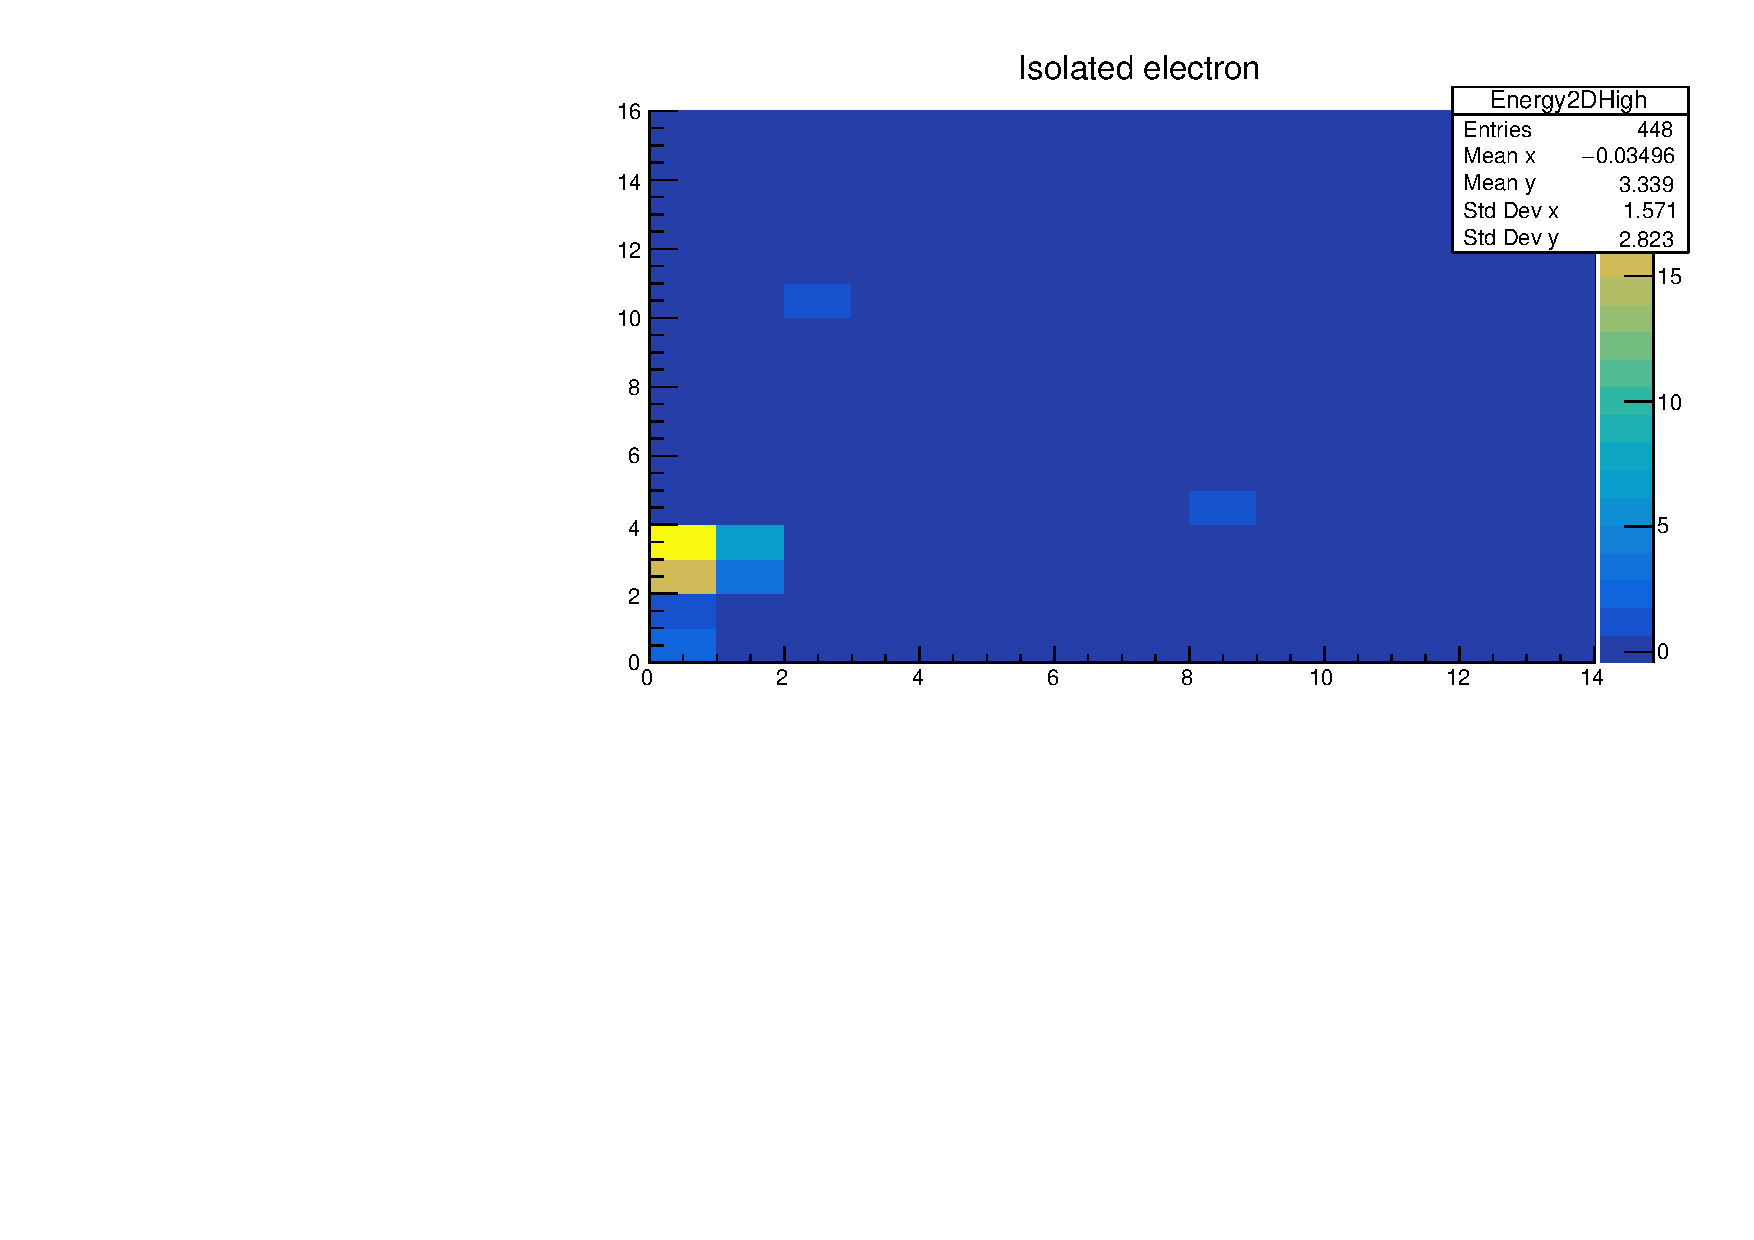
\includegraphics[width=\textwidth]{electronhist.pdf}
\end{minipage}
\begin{minipage}{0.45\textwidth}
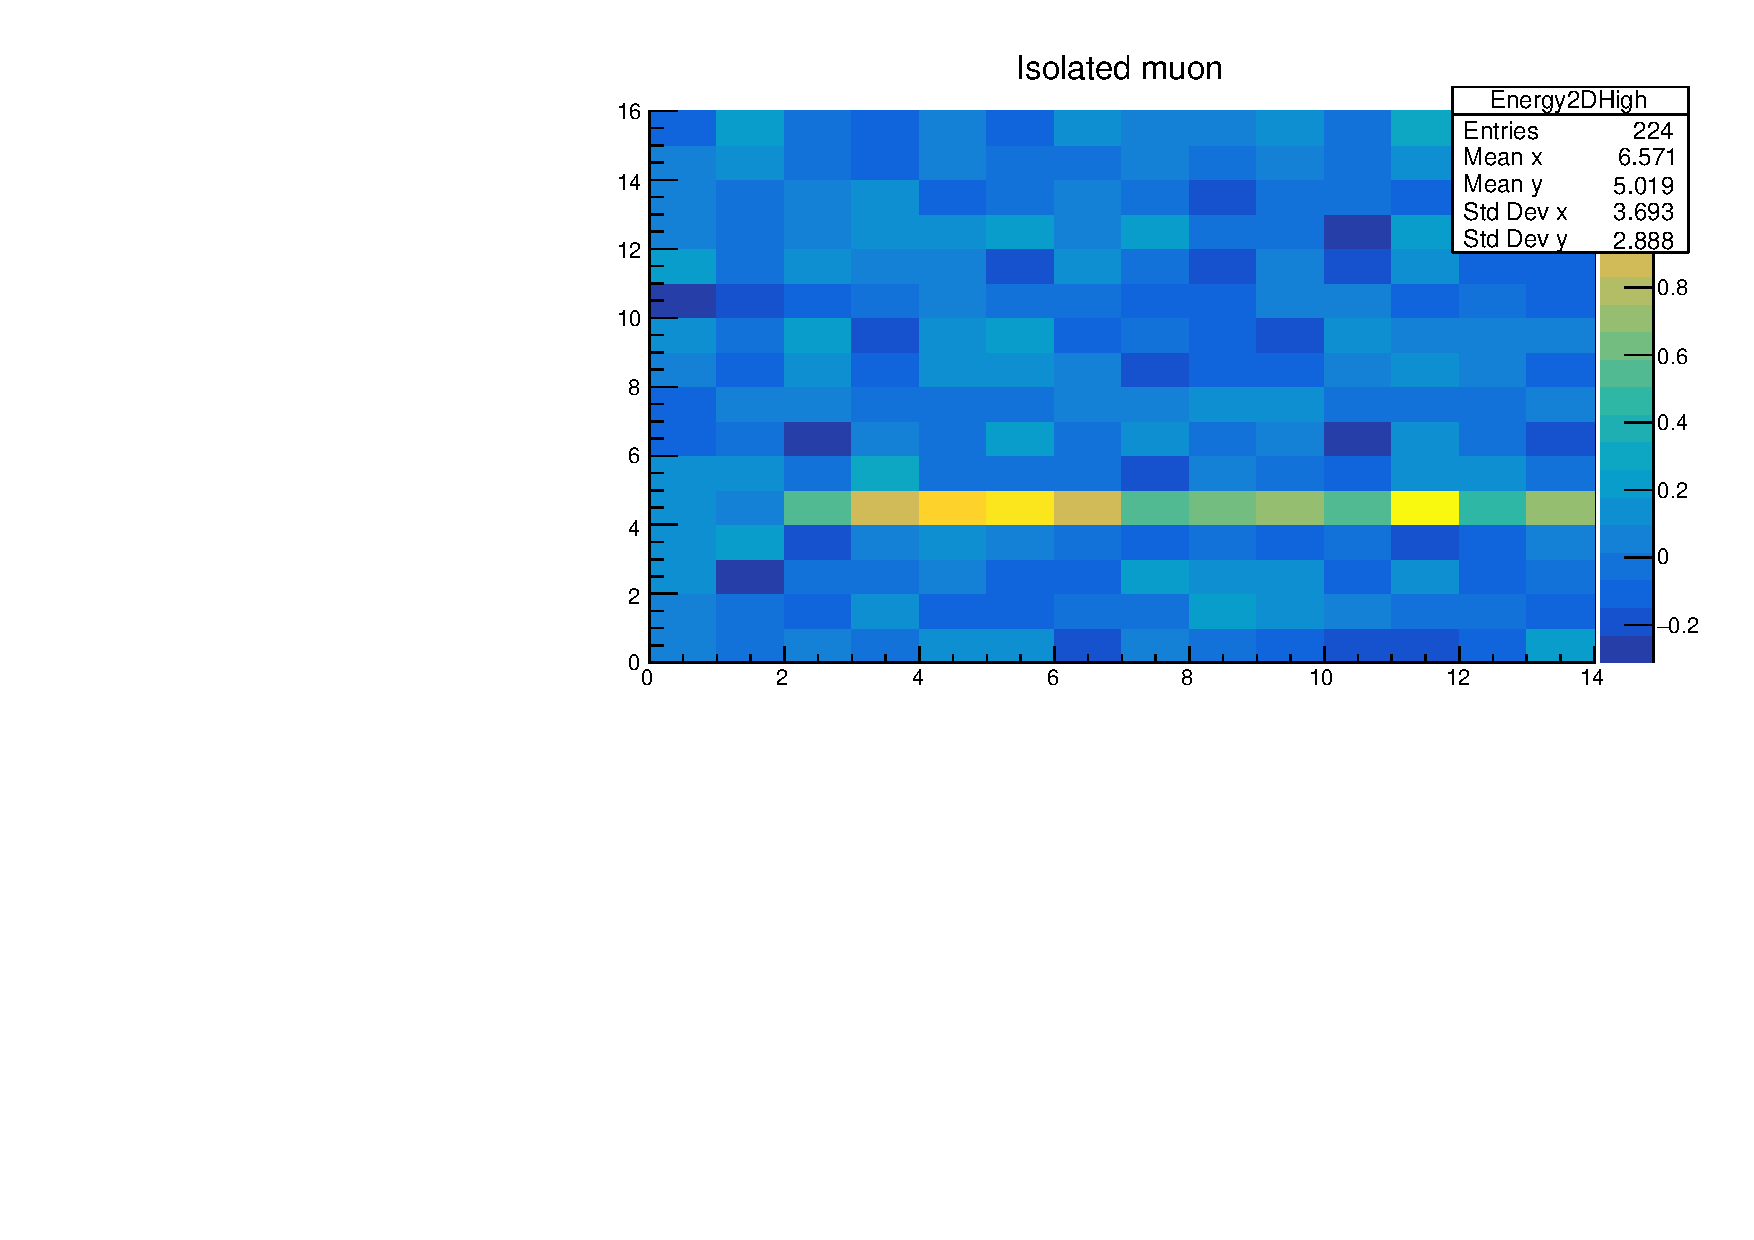
\includegraphics[width=\textwidth]{muonhist.pdf}
\end{minipage}
\end{minipage}
\begin{minipage}[b]{0.95\textwidth}
\begin{minipage}{0.45\textwidth}
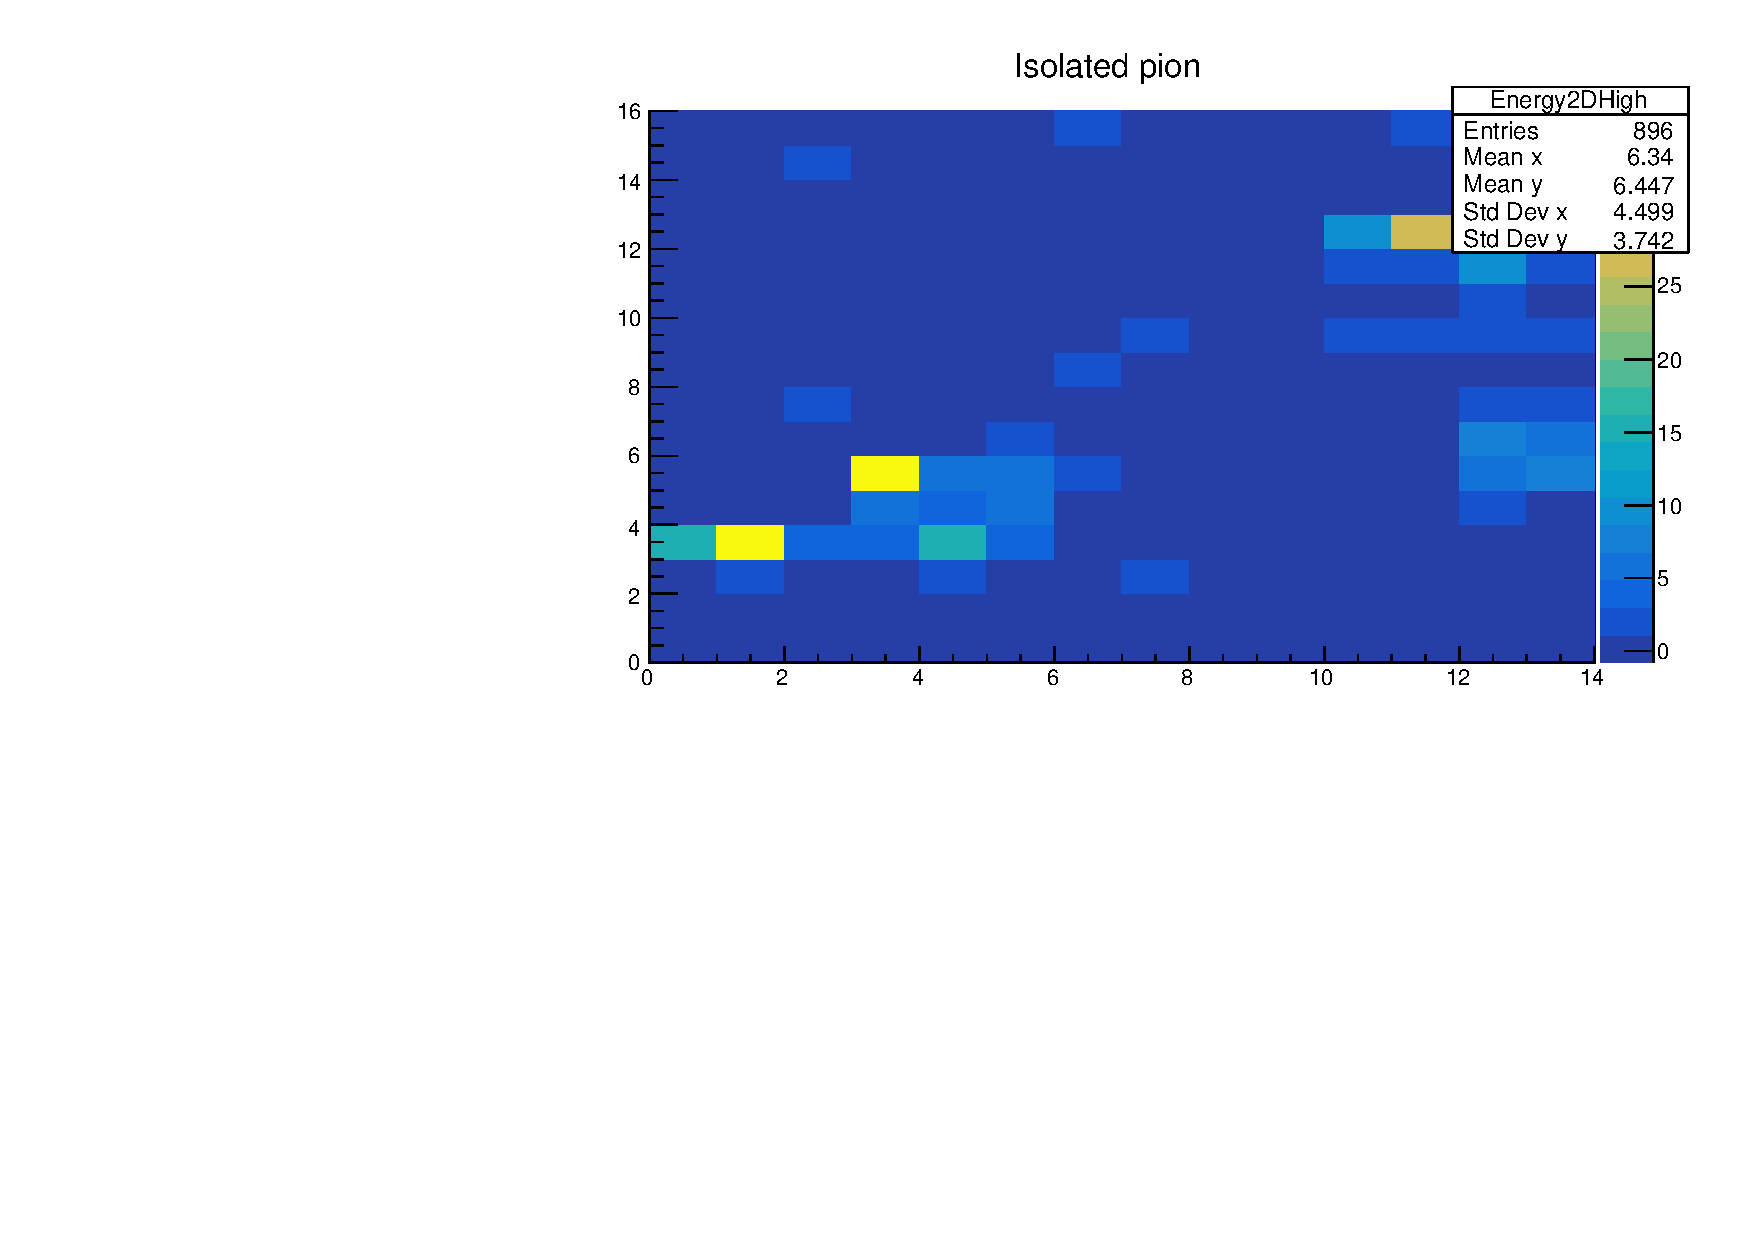
\includegraphics[width=\textwidth]{pionhist.pdf}
\end{minipage}
\begin{minipage}{0.45\textwidth}
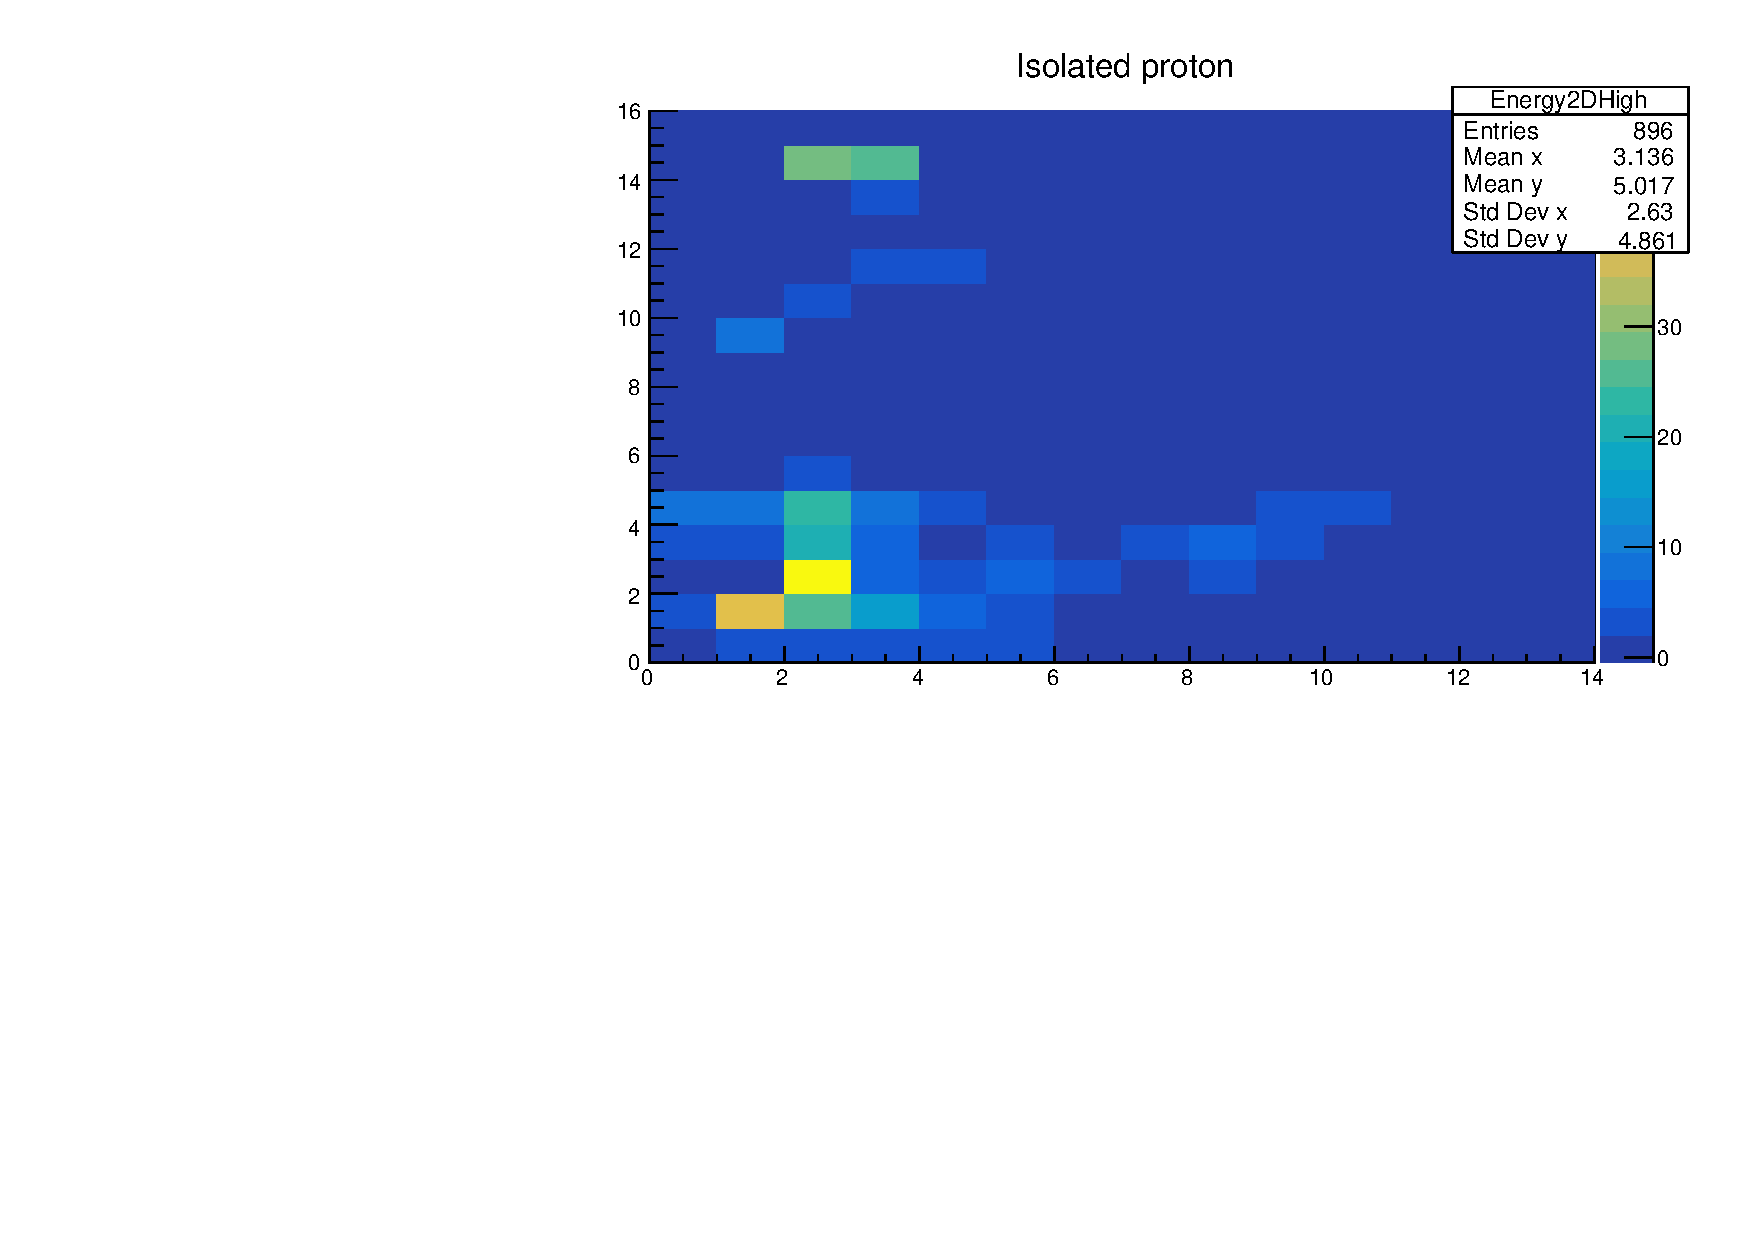
\includegraphics[width=\textwidth]{protonhist.pdf}
\end{minipage}
\end{minipage}
\caption{Energy deposit of single particles travelling through CASTOR. An electron or photon (upper left) deposits its whole energy in the electromagnetic sections, while a muon travels with only a little energy loss through every section (upper right). The signals of pions and protons is spread wider and reaches into the hadronic sections of the calorimeter (lower left and right). The data is generated by EPOS.}
\label{signals}
\end{figure}

As seen in fig. \ref{signals}, the energy deposited in CASTOR by different particles varies much. In different events particles with very different energies are created. For example the kinetic energy of a proton can be between one and several thousand GeV. To learn that these very different signals are generated by the same particle type would pose a challenge for the neural network. Every histogram is therefore normalized to 1 in signal amplitude. 
\begin{table}
\centering
\caption{Number of isolated particles travelling through CASTOR in 500.000 Monte Carlo generated events. If not specified otherwise, the numbers include the particle and the antiparticle. As can be seen, hadrons and electrons/photons dominate the spectrum.}
\sffamily
\begin{tabular}{cc |cc }
\hline
Leptons/Bosons & Count & Hadrons & Count \\ \hline
Photon & 170047 & $\pi^+$ & 106904 \\
Positron & 243 & $\pi^-$ & 103648 \\
Electron & 250 & $K^+ / K^-$ & 27591 \\
Muon & 29 & Proton & 15782\\
$\nu_{\mu}$ & 27 & Neutron & 15232 \\
$\nu_e$ & 11 & $K^0_L$ & 13604 \\
$\nu_{\tau}$ & 1 &  $\Lambda$ & 5308\\
& & $\Sigma^+$ & 2016 \\
& & $\Sigma$ & 1993 \\
& & $\Sigma^-$ & 1993 \\
& & $K^0_s$ & 1323 \\
& & $\Xi^0$ & 511 \\
& & $\Xi^-$ & 471 \\
& & $\Omega^-$ & 16 \\
 \hline
\end{tabular}
\label{particlecounts}
\end{table}
\section{Network design}
The energy deposit histograms of CASTOR can be treated as pictures with 16 to 14 pixels and varying amounts of colour intensity. To design a neural network which can classify events into particle categories techniques in image recognition should be used. In normal classification problems convolutional layers with a small and quadratic kernel size are used. Here the information given by the underlying physics can be used to the advantage of the network. 

As particles reach the calorimeter from the left, it is not useful to use small kernel sizes to cover the whole image. Small, light particles are normally contained in one tower or at most two. Therefore convolutional layers with kernel sizes of one or two towers, meaning one or two pixels in the height and 7 or 14 in the width, should be able to recognize the important features of the tracks. Several layers, each with kernel sizes with a width of 14 pixels but varying heights are concatenated in the beginning of the network. In the deeper layers of the network, smaller kernel sizes can be used, since the convolution shrinks the size of the signal travelling through the neurons. In fig. \ref{convnet} the network structure is shown. Because of the large kernel sizes in the beginning, the size of the data volume shrinks quickly. Max pooling was therefore omitted as too much information was lost due to the rather small input size. Deeper networks with more hidden layers have been tested but showed no advantage in accuracy. Deeper networks only need more computing time and have a higher tendency to overfit as more free parameters are available. 

\begin{figure}
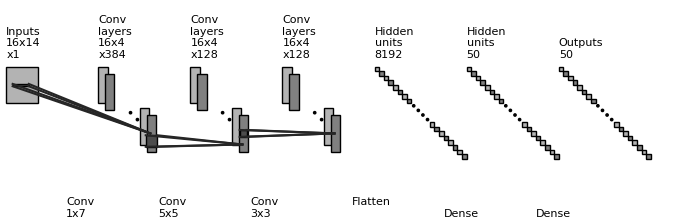
\includegraphics[scale=0.85]{convnet_fig.png}
\caption{The network design for the convolutional neural network. The first convolutional layer is composed out of kernel sizes of (1, 7), (2, 7) and (3, 7). This was omitted for a clearer picture. To reduce overfitting, dropout is used between after the first convolutional layer and before and after the first dense layer, each with a probability of 0.5. \protect \footnotemark}
\label{convnet}
\end{figure}

\section{Monitoring}
For monitoring the progress of a neural network, the first important feature is the loss function. As the classification problem is a multi-label classification, the loss function used here is the binary crossentropy loss. Every epoch it is calculated for the training and for the validation data set. Both variables need to decrease during the training. To determine if the input is correctly put into the network the first step was to train without any dropout or pooling layers. The network should overfit on the training set if given enough time. In fig. \ref{overfitacc} the loss and the accuracy of the training while overfitting can be seen.
\footnotetext{This figure is generated by adapting the code from \url{https://github.com/gwding/draw_convnet}}
\begin{figure}
\centering
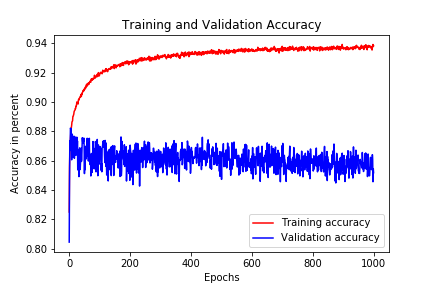
\includegraphics[scale=0.8]{trainvalacc.png}
\caption{Training and validation accuracy. Both start at roughly the same percentage, but as training goes on, the training accuracy increases constantly. The validation accuracy does not change or even decreases a little. This is a classic overfitting effect.}
\label{overfitacc}
\end{figure}
As standard networks normally deal with multi-class and not multi-label problems, it proved to be useful to additionally monitor variables commonly used in classification problems. Here recall and precision were implemented \cite{rijsbergen}. With recall, the false negatives are taken into account, while precision monitors the false positives. Recall is also called the sensitivity of a network and is calculated by
\begin{equation}
\mathrm{Recall} = \frac{tp}{tp + fn} \quad ,
\label{recall}
\end{equation}
where tp stands for true positive, tn for false negative. The recall therefore is the fraction of true positive labels over all actually positive labels. In the case of all labels being correctly predicted, the recall is 1. Precision is also referred to as the positive predictive value. It is the rate of all correctly classified positive labels over all positively predicted labels.
\begin{equation}
\mathrm{Precision} = \frac{tp}{tp + fp}
\end{equation}
The nomenclature is the same, tp for true positives and fp for false positives. When all labels are correctly predicted, the precision also equals 1.

The precision and the recall can be calculated separately for the different categories. It can be easily monitored if the networks has more problems recognizing one category over the others. 

%Another number which was monitored was the number of falsely labelled electrons. It was obvious after a few training sessions that the network had most problems classifying electrons. A counter of the falsely labelled electrons was therefore implemented in the callbacks. With y$_{\mathrm{true}}$ as the true labels and y$_{\mathrm{pred}}$ as the predicted labels, the counter worked as seen below.
%\begin{equation}
%\mathrm{count} = (1 - y_{\mathrm{true}}) \cdot y_{\mathrm{pred}} - (1 - y_{\mathrm{pred}}) \cdot y_{\mathrm{true}}
%\end{equation}
%It is the same as the crossentropy loss without the logarithm, but with two main differences. The first one is that here not the predicted probabilities are used as input put the absolute prediction. That means if y$_{\mathrm{pred}}$ is higher than 0.5 it is rounded to 1, lower than 0.5 means being rounded to 0. The second one is it being a difference rather than a sum. This way if the number is negative, the network has more false negatives than false positives, if it is positive, more false positives than negatives. 
\section{Evaluation}
In the process of training it became apparent that no real physical features were being learned by the network. The training loss decreased but the validation remained constant over several hundred epochs (fig. \ref{trainvalloss}). As mentioned before, without  regulations the network overfitted on the training data without problem. This lead to reevaluating the input data, as it seemed to be difficult for the network to generalize the underlying physical laws. 

\begin{figure}
\centering
\begin{minipage}{0.45\textwidth}
\centering
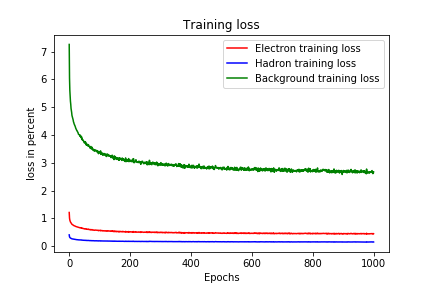
\includegraphics[scale=0.45]{trainloss.png}
\end{minipage}
\begin{minipage}{0.45\textwidth}
\centering
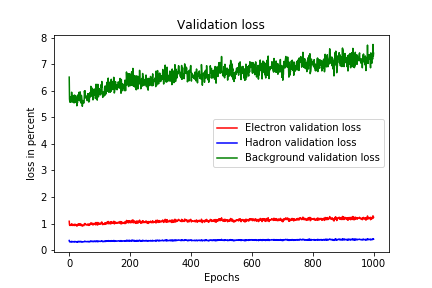
\includegraphics[scale=0.45]{valloss.png}
\end{minipage}
\caption{Training and validation loss for single particles. The training loss behaves exactly as it is supposed to, decreasing gradually during training. The validation loss shows that the network is not generalizing properly. It is remaining constant or even increasing, showing that the error rates get higher.}
\label{trainvalloss}
\end{figure}

One problem was the definition of background events. Since at first only isolated particles were considered, background events could also contain hadrons or electrons and photons, just not in the right distance to other particles travelling through CASTOR. The background category therefore contained input data which were not distinguishable from an photon or hadron event. To solve this problem, two different approaches were chosen. The first one was to completely ignore the background category and turn the classification into a binary problem, only distinguishing between electromagnetic particles, photons and electrons, and hadrons. The second was the redefinition of the background category, where only true background was used. True background meant, that no particle with an energy higher than 3 GeV had travelled through CASTOR in the corresponding signal. To further simplify the classification, only single particles were used, meaning that one particle per event crossed CASTOR. In tab. \ref{singleparticles} are the particles belonging to this data set. The background category consists mostly of no particles, which is not shown here. As single particles are rarer than isolated particles, two million events were evaluated. Still the number of useful histograms is smaller than with isolated particles, where 500.000 events were used.

\begin{table}
\centering
\caption{Single particles crossing through CASTOR. The particles in the background category are no single particles but have an energy less than 3 GeV. Two million events were evaluated.}
\sffamily
\begin{tabular}{cccc}\hline
Particle & Electromagnetic Class & Hadronic Class & Background Class \\ \hline
$\Lambda$ & 0 & 641 & 0 \\
Proton & 0 & 1915 & 0 \\
Neutron & 0 & 2355 & 0 \\
Electron  & 64 & 0 & 11 \\
Photon & 18327 & 0 & 80 \\
Pi$^{+-}$ & 0 & 25292 & 3 \\ 
K$^{+-}$ & 0 & 3608 & 0 \\
K$_l$ & 0 & 1769 & 0 \\
K$_s$ & 0 & 1812 & 0 \\
$\Omega^-$ & 0 & 3 & 0 \\
$\Xi^0$ & 0 & 53 & 0 \\
$\Xi^-$ & 0 & 52 & 0 \\
$\Sigma^+$ & 0 & 263 & 0 \\
$\Sigma^-$ & 0 & 384 & 0 \\
\hline
\end{tabular}
\label{singleparticles}
\end{table}


As precision and recall were implemented as callbacks, their value was returned after every epoch. In the first few training sessions the monitoring of these showed that while the mean loss decreased and the accuracy increased, the recall especially of electrons remained really low. To counteract this, the binary crossentropy loss was defined as a separate function. The crossentropy is the sum of two parts, one evaluating and penalizing the number of false positives, the other watching the number of false negatives. As recall, as seen in eq. \enquote{\ref{recall}}, evaluates the false negatives, they were stronger penalized than the false positives.

\subsection{Comparison between different data inputs}

To evaluate the possible applications and limits of the event classification with the help of a neural network, several data sets have been used and compared. As the first idea was to classify isolated particles, one dataset is composed of isolated electromagnetic particles, isolated hadronic particles and background, in which no isolated particle crosses CASTOR. All particles included in this data can be seen in table \ref{particlecounts}. As the background definition for this data type was difficult and the distinguishing between events with more than one particle to those with only one also seemed to worsen the performance of the network, single particles were introduced. Only events in which just one particle had crossed through CASTOR were counted here. To also better define the background class, events with particles no higher than 3 GeV or no particle in CASTOR	were included in this class. At last, a binary classification was tried, excluding the background completely. For every data type, the training and the validation loss function can be seen in fig. \ref{lossall}. The expected result would be that the network performs worse on isolated particles since the distinction between background and electromagnetic/hadronic particles was not clear. Several events could also fall in both the electromagnetic and the hadronic class, which was more difficult to recognize. As can be seen in fig. no analysis behaves at it should. The training loss decreases exponentially, which is the expected behaviour. The validation loss remains constant or increases. This should not happen as dropout of 0.5 is used during all training time. Increasing dropout had no effect on the training. As the training loss functions correctly, it can be assumed that the implementation of the network is right. It seems to be unable to identify physical features which correctly classify the events. A hadronic process is more easily identified judging by the relatively small loss function. 

\begin{figure}
\centering
\begin{minipage}{0.45\textwidth}
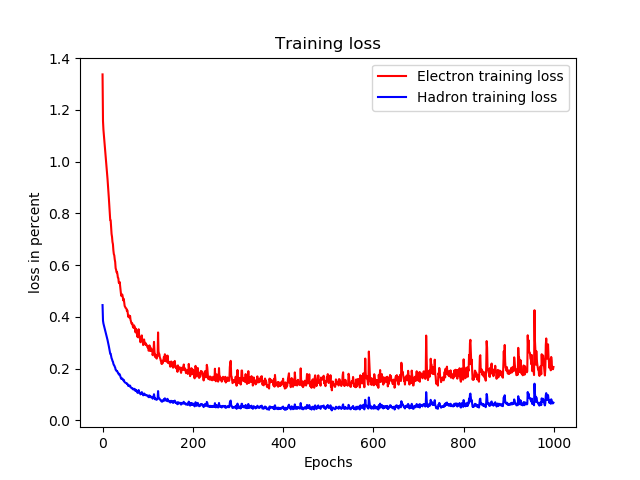
\includegraphics[width=7cm]{trainlossbinary.png}
\end{minipage}
\begin{minipage}{0.45\textwidth}
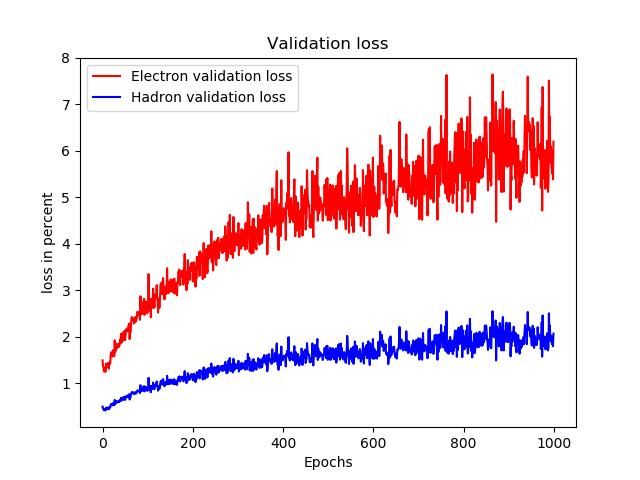
\includegraphics[width=7cm]{vallossbinary.png}
\end{minipage}
\\
\begin{minipage}{0.45\textwidth}
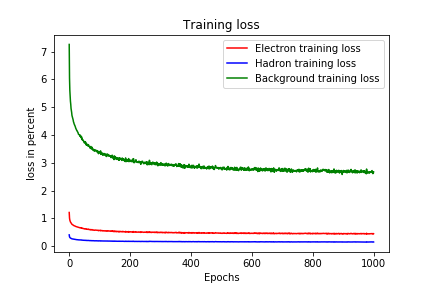
\includegraphics[width=7cm]{trainloss.png}
\end{minipage}
\begin{minipage}{0.45\textwidth}
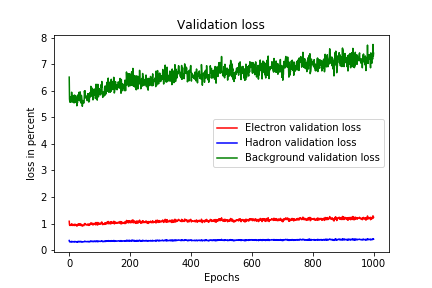
\includegraphics[width=7cm]{valloss.png}
\end{minipage}
\\\begin{minipage}{0.45\textwidth}
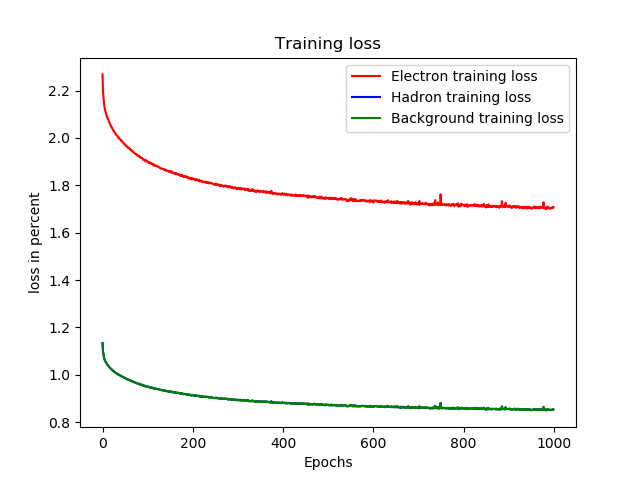
\includegraphics[width=7cm]{trainlossisolated.png}
\end{minipage}
\begin{minipage}{0.45\textwidth}
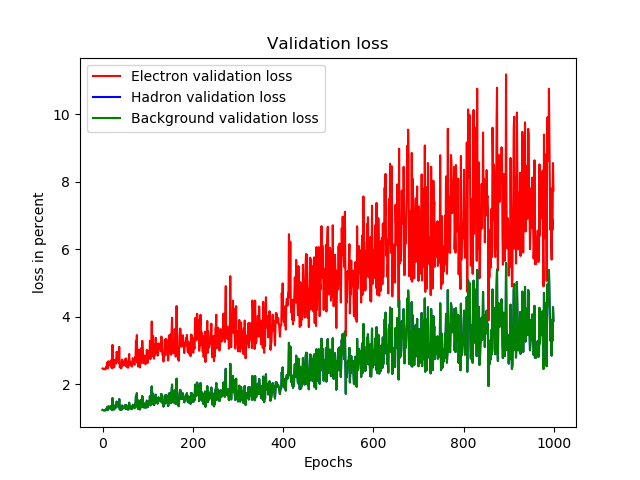
\includegraphics[width=7cm]{vallossisolated.png}
\end{minipage}
\caption{Training and validation loss for different data sets. At first the binary classification is shown, then the single particles and at last the isolated particles. The correct tendency for the loss function to decrease is seen in every training figure. The validation loss behaves not as it should. It seems to forget what it learned.}
\end{figure}

\begin{figure}
\centering
\begin{minipage}{0.45\textwidth}
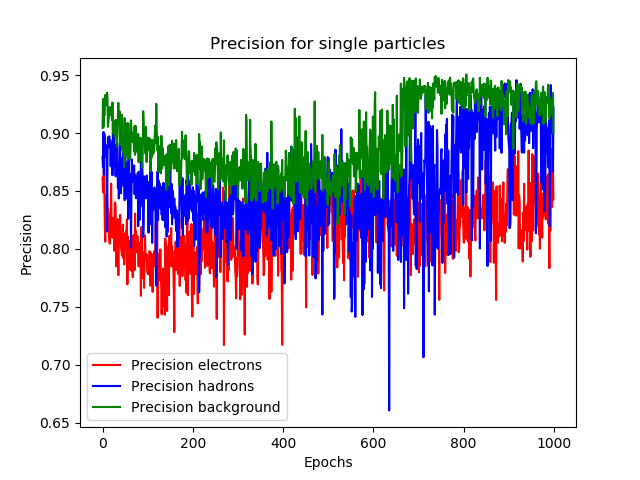
\includegraphics[width=7cm]{precisionsingle.png}
\end{minipage}
\begin{minipage}{0.45\textwidth}
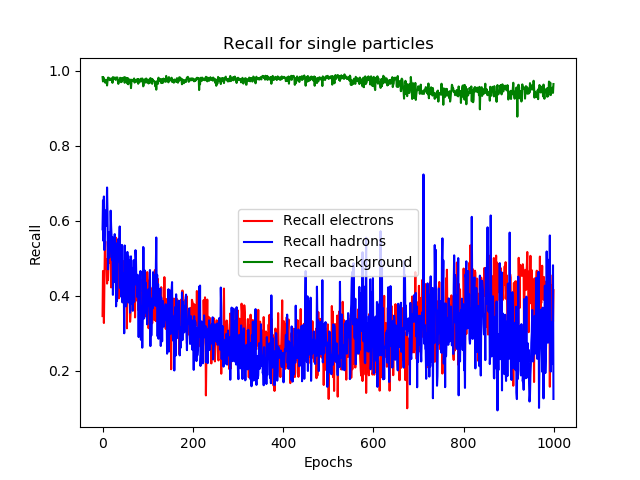
\includegraphics[width=7cm]{recallsingle.png}
\end{minipage}
\caption{Precision and recall for single particles. The precision is rather high, false positives are therefore seldom. In comparison, recall is low for electrons and hadrons. Many times the network falsely labels an event as not belonging to one of these categories but rather to the background or no class.}
\label{lossall}
\end{figure}

The single particles have the most constant performance on the validation data set but it still seems to increase during training time. The last set in fig. \ref{lossall} is the training with isolated particles. For unknown reasons the background loss function behaves exactly the same as the hadron loss function, during training as well as during validation. 
\subsection{Performance on actual data}
To see how the network performed on actual data after training, two runs with proton-proton collisions at $\sqrt{s}$ = 13 TeV with very low luminosity were evaluated. The low luminosity was useful to ensure that a high number of events contained isolated or single particles. To assess the performance of the network, the ratio of electromagnetic energy deposit contained in the first two sections of every tower to hadronic energy deposit in the following 14 sections was calculated. The energy ratio E$_{\mathrm{em}}$/(E$_{\mathrm{em}}$ + E$_{\mathrm{had}}$)is shown in the histograms in fig. \ref{ratio}, in comparison to actual electromagnetic and hadronic events and their ratio made by Monte Carlo simulations by EPOS. 
\begin{figure}
\centering
\begin{minipage}{0.45\textwidth}
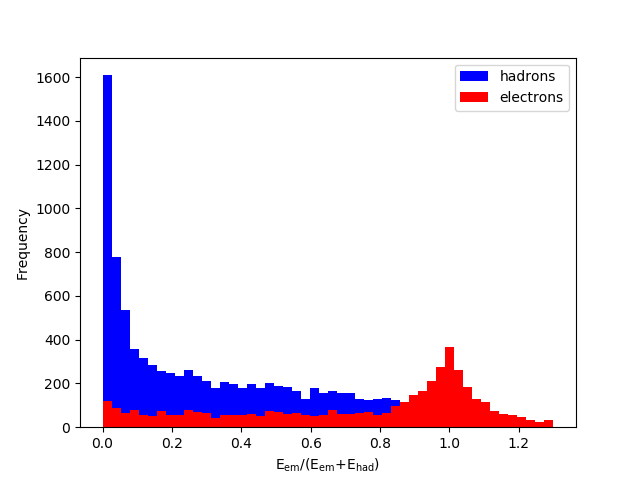
\includegraphics[width=7cm]{ratio.png}
\end{minipage}
\begin{minipage}{0.45\textwidth}
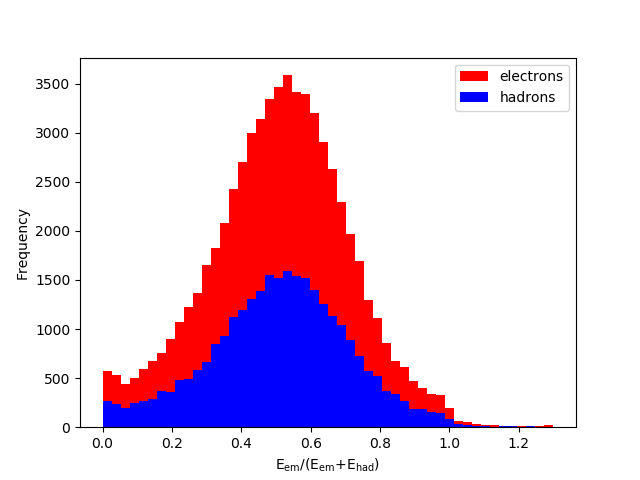
\includegraphics[width=7cm]{emhadbinary.png}
\end{minipage}
\\
\begin{minipage}{0.45\textwidth}
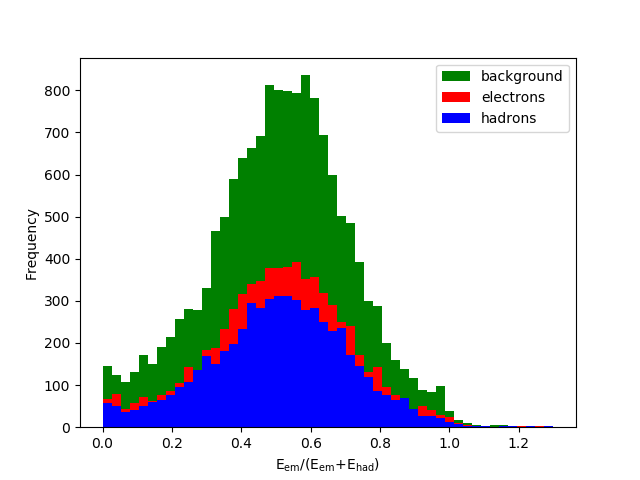
\includegraphics[width=7cm]{emhadsingle.png}
\end{minipage}
\begin{minipage}{0.45\textwidth}
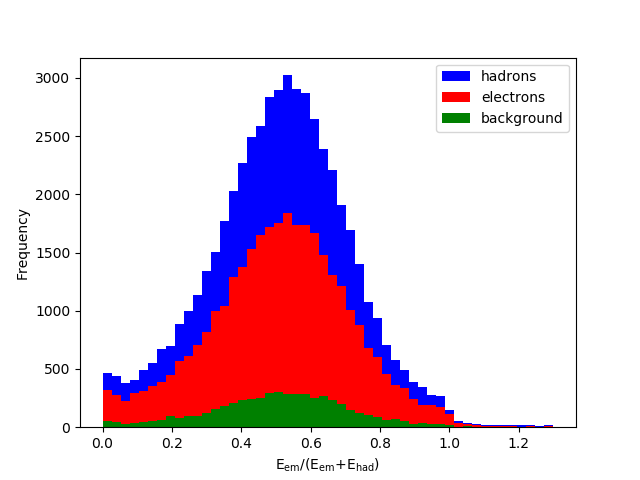
\includegraphics[width=7cm]{emhadisolated.png}
\end{minipage}
\caption{Electromagnetic to hadronic energy in the different categories. The figure on the upper left are simulated events with single electromagnetic and hadronic particles. On the upper right hand side are the ratios based on the prediction trained on binary particles. On the lower left hand side are the predictions based on single particles, on the lower right hand side the predictions based on the isolated particles.}
\label{ratio}
\end{figure}

For electromagnetic events this ratio should be nearly 1, while for hadronic events a peak at 0 is to be expected. In the simulated events this behaviourism is very obvious. There are two peaks in the histogram, one for electromagnetic and one for hadronic events. In the predicted events the tendency cannot be seen. In the real events classified by the network the energy distribution is the same for all predicted categories. As most events do not contain single or isolated particles the energy ratio is centered around 0.5. This is due to several particles per event travelling through CASTOR. Interesting is the varying amount of events predicted as CASTOR by the network trained on single and on isolated particles. As events with isolated particles can also contain several particle tracks at once more events fall into the electromagnetic or hadronic category. For single particles more events are classified as belonging to background since several particle events were excluded as training events for the other two categories.
 
The neural network is unable to correctly identify a high number of events. As in real data single or isolated particles can not be separated, many events contain several particles crossing CASTOR. This is difficult for a network to classify correctly. To see if the network is classifying at least some events accurately, events belonging to one class with a probability of at least 80 \% have been picked out. These events were then again displayed as a two dimensional histogram. An electromagnetic and a hadronic event is shown in fig. \ref{electron}. Both have been identified by the neural network trained on single particles, the networks trained on binary and isolated particles identified similar events. The signature tracks of both particle types are clearly visible. The electromagnetic particle leaves a short track, depositing its energy in the first two sections of one or two towers. A hadronic particle leaves a wider track, decaying into lighter particles, which deposit their energy throughout the detector.
\begin{figure}
\centering
\begin{minipage}{0.45\textwidth}
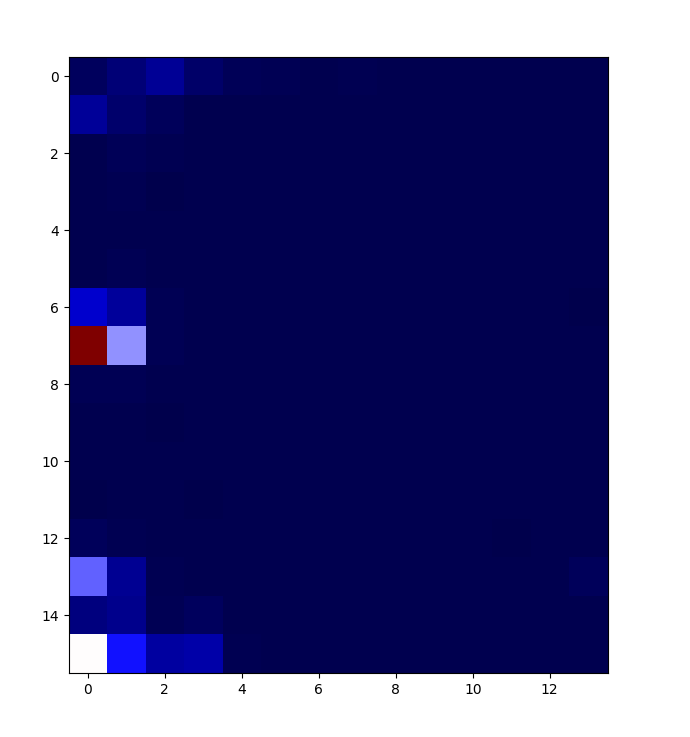
\includegraphics[width=6cm]{electron.png}
\end{minipage}
\begin{minipage}{0.45\textwidth}
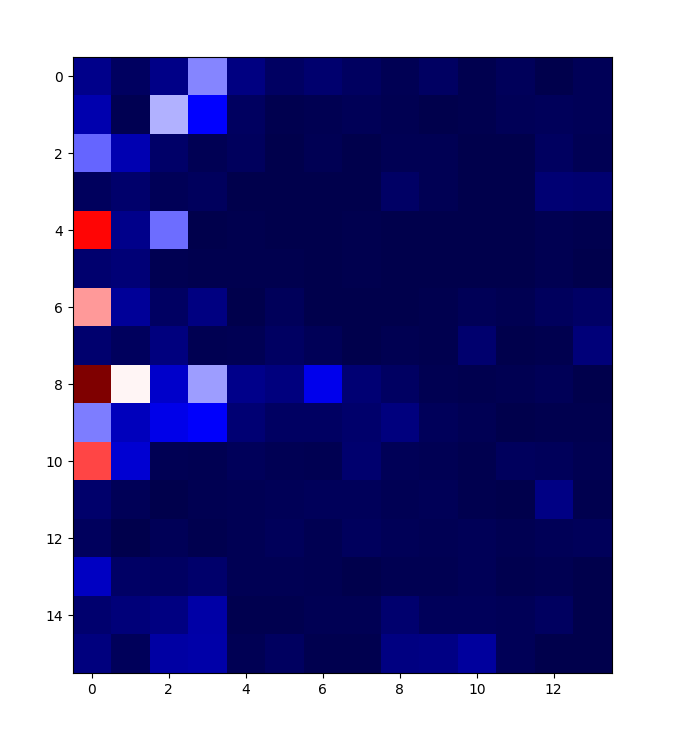
\includegraphics[width=6cm]{hadron.png}
\end{minipage}
\caption{One electromagnetic and one hadronic event with a probability higher than 80 \%. On the left the short track of an electron or photon can be seen, depositing nearly all energy in the first two sections. On the right is the wider signature of a hadron.}
\label{electron}
\end{figure}

At least a few events can be correctly identified by the neural network. The performance is not dependent on the data type used for training. Obvious particle tracks which are left by single particles can be recognized by a trained network. Overlapping signals are difficult for the network to discern and are then randomly put into one category. In real data isolated or single particles happen seldom. This explains the incorrectly behaving electromagnetic to hadronic ratio.

\subsection{Error analysis}
After several training cycles the loss function of the network still did not converge. Several possible causes for this failure have been mentioned and rectified, such as the definition of background events, very low recall and the network design. But even with only two categories, electron/photon and hadronic events, the loss function continued to show erratic behaviour. The network only performed well on very clear tracks. Events with several particles were not identified correctly. There are many possibilities which caused the poor classification, a few are going to be evaluated here.

The first one is the lack of training time. Neural networks which perform as well or even exceed human performance have an average training time of three weeks. This was not possible during this thesis as a continuous evaluation of the network's performance was needed. 

The second one is the actual distinction between hadronic and electromagnetic events with only the energy deposit as input data. As hadronic events can also cause electromagnetic showers the input signals can seem similar. If several particles cross CASTOR in one event, the overlapping signals can be difficult to distinguish. 

At last using conventional convolutional layers, important physical information gets lost. As the particles always enter the calorimeter from the left side, layers with higher weights and therefore more emphasis on the first sections could perform better than those used here. Convolutional layers share the same weights across the whole input, so no part is highlighted. This is advantageous in classic image recognition, but not for event classification in a calorimeter. 
    \chapter{Summary}
    CASTOR is a electromagnetic and hadronic calorimeter, which measures the very forward region of CMS. In future it can be used to detect and identify new particles such as strangelets. For this a full event classification of known particles has been tried using neural networks. In this thesis only detector data has been used without reconstruction of particle data. To simplify the analysis, only particle types were tried to separate. Three classes were implemented, electromagnetic particles, which included photons and electrons, hadronic particles, mostly pions, and background which was defined differently for different data sets. The implementation of the network was done with keras, using tensorflow, a python based machine learning framework, as a backend. As calorimeter data represented by a histogram of the energy deposit per section can be seen as an image, classical image recognition methods were applied. This meant a network consisting mostly of convolutional layers, which can detect spatially local features better and faster than conventional neural networks. \newline
The network was trained on three different data sets, isolated particles, single particles and a binary classification, omitting the background category. Several network designs have been tested, finally deciding on a network with 6 hidden layers. Deeper networks have not shown a better performance. The network performance was continuously tested on validation data to oversee the learning progress and to possibly prevent overfitting. In the end the network did not perform very well on either data set. Used on real data it was able to identify events correctly, which had a very high probability of belonging to one class. Those events which bordered on 50 \% probability were often wrong and contributed to the poor performance of the network. This may be due to the fact that physical information was not conveyed through the classic convolutional layers. The particles detected by CASTOR always enter the calorimeter from the same direction. Therefore more emphasis should be placed on the left sections of every tower in further analyses. \newline
In conclusion, the application of neural networks in particle physics is vast and has been shown in several other experiments. For a full event classification, with the limited methods used in this thesis, using only calorimeter data is a major challenge for the network. A significant preprocessing of the data is needed and the network does not easily reach the performance of classical methods. To better the classification either additional data of other detectors can be included, to make the identification easier, or customized network layers should be designed. The physical information, which can be implemented through the network design or by preprocessing the data, should increase the ability to classify events. 

   % \emptychapter[3]{ROOT Routines}     % usage: \emptychapter[page displayed 
                                        %        in toc]{name of the chapter}



   % \chapter{Conclusions}
    %\lipsum[1-5]


    % appendix for more or less interesting calculations
    %\Appendix
    %\chapter*{\appendixname} \addcontentsline{toc}{chapter}{\appendixname}
    % to make the appendix appear in ToC without number. \appendixname = 
    % Appendix or Anhang (depending on chosen language)
    %\section{First Appendix Section}
Wonderful Appendix!

\lipsum[1-5]
 %\cleardoublepage



    % Bibliography
    \TheBibliography

    % BIBTEX
    % use if you want citations to appear even if they are not referenced to: 
    % \nocite{*} or maybe \nocite{Kon64,And59} for specific entries
    \nocite{*}
    \bibliographystyle{ieeetr}
    \bibliography{lit}

    % THEBIBLIOGRAPHY
    %\begin{thebibliography}{000}
    %    \bibitem{ident}Entry into Bibliography.
    %\end{thebibliography}
\end{document}
